\pdfminorversion=4
\documentclass[11pt,a4paper]{report} 
% Alternativ für doppelseitigen Ausdruck (nur bei > 60 Seiten sinnvoll)
%\documentclass[11pt,a4paper,twoside,openright]{report}

% Deutsch
\usepackage[german]{babel} % deutsch und deutsche Rechtschreibung
\usepackage[utf8]{inputenc} % Unicode Text 
\usepackage[T1]{fontenc} % Umlaute und deutsches Trennen
\usepackage{textcomp} % Euro
\usepackage[hyphens]{url}
% statt immer Ab\-schluss\-ar\-beit zu schreiben
% einfach hier sammeln mit -. 
\hyphenation{Ab-schluss-ar-beit}
% Vorsicht bei Umlauten und Bindestrichen
\hyphenation{Ver-st\"ar-ker-aus-gang}
 % eigene Hyphenations, die für das Dokument gelten
\usepackage{amssymb} % Symbole
\usepackage{enumitem}
\usepackage{tabularx}


%% Fonts, ein kompletter Satz an Optionen
% Times New Roman, gewohnter Font mit ok tt und serifenlos
%\usepackage{mathptmx} 
%\usepackage[scaled=.95]{helvet}
%\usepackage{courier}
% Palatino, mal was anderes, auch mit ok tt und serifenlos
% empfohlen
\usepackage{mathpazo} % Palatino, mal was anderes
\usepackage[scaled=.95]{helvet}
\usepackage{courier}
% New Century Schoolbook sieht auch nett aus (macht auch tt und serifenlos)
%\usepackage{newcent}

% zusätzlich: Default serifenlos mit Helvetica 
% ich kann es nicht mehr sehen...
%\renewcommand{\familydefault}{\sfdefault}

\usepackage{microtype}

% Bilder und Listings
\usepackage{graphicx} % wir wollen Bilder einfügen
\usepackage{subfig} % Teilbilder
\usepackage{wrapfig} % vielleicht doch besser vermeiden
\usepackage{listings} % schöne Quellcode-Listings
% ein paar Einstellungen für akzeptable Listings
\lstset{basicstyle=\sffamily, columns=[l]flexible, mathescape=true, showstringspaces=false, numbers=left, numberstyle=\tiny}
\lstset{language=python} % und nur schöne Programmiersprachen ;-)
% und eine eigene Umgebung für Listings
\usepackage{float}
\newfloat{listing}{htbp}{scl}[chapter]
\floatname{listing}{Listing}

% Seitenlayout
%\usepackage[paper=a4paper,width=14cm,left=35mm,height=22cm]{geometry}
\usepackage[paper=a4paper,width=14cm,height=22cm]{geometry}
\usepackage{setspace}
\linespread{1.15}
\setlength{\parskip}{0.5em}
\setlength{\parindent}{0em} % im Deutschen Einrückung nicht üblich, leider

% Seitenmarkierungen 
\newcommand{\phv}{\fontfamily{phv}\fontseries{m}\fontsize{9}{11}\selectfont}
\usepackage{fancyhdr} % Schickere Header und Footer

\pagestyle{fancy}
\renewcommand{\chaptermark}[1]{\markboth{#1}{}}
\renewcommand{\sectionmark}[1]{\markright{#1}}
\fancyhead[LO]{\phv \nouppercase{\leftmark}}
\fancyhead[RE]{\phv \nouppercase{\rightmark}}
\fancyhead[RO,LE]{\phv \thepage}
\fancyfoot[C]{\ } % Seitenzahl unten nur Kapitel


% Theorem-Umgebungen
\newtheorem{definition}{Definition}[chapter]
\newtheorem{satz}{Satz}[chapter]
\newtheorem{lemma}[satz]{Lemma} % gleicher Zähler wie Satz
\newtheorem{theorem}{Theorem}[chapter]
\newenvironment{beweis}[1][Beweis]{\begin{trivlist}
\item[\hskip \labelsep {\textit{#1 }}]}{\end{trivlist}}
\newcommand{\qed}{\hfill \ensuremath{\square}}

% Inhaltsverzeichnis
\setcounter{tocdepth}{1}
\setcounter{secnumdepth}{2}

% Quellen teilen
\usepackage{bibtopic} 

% Hochschule Logo, noch nicht perfekt
\usepackage{hsrmlogo}

% Spezialpakete
\usepackage{epigraph}
\setlength{\epigraphrule}{0pt} % kein Trennstrich

% damit wir nicht so viel tippen müssen, nur für Demo 
\usepackage{blindtext} 

% Zum Zeigen von Fehlern
\usepackage{soul}
\newcommand*\falsch{\st}

% Links im PDF
\usepackage{hyperref}
\hypersetup{
    colorlinks=true,
    citecolor=black,
    filecolor=black,
    linkcolor=black,
    urlcolor=black
}

% Kommentare
\usepackage{comment} % alle Pakete und Einstellungen	
\usepackage{hyperref}
% Hier anpassen 
\newcommand{\titel}{Entwurf, prototypische Implementierung und Evaluation eines Sicherheitskonzepts für die Authentifizierung und Autorisierung von Fernzugriffen auf eine Automatisierungsanlage}
\newcommand{\kurztitel}{Template Abschlussarbeit}
\newcommand{\autor}{Kevin Sapper}
\newcommand{\datum}{14. Oktober 2014} % Abgabedatum
\newcommand{\ort}{Wiesbaden}
\newcommand{\referent}{Prof.\ Dr.\ Reinhold Kröger}
\newcommand{\korreferent}{Prof.\ Dr.\ Martin Gergeleit}

\newenvironment{conditions*}
  {\par\vspace{\abovedisplayskip}\noindent
   \tabularx{\columnwidth}{>{$}l<{$} @{\ : } >{\raggedright\arraybackslash}X}}
  {\endtabularx\par\vspace{\belowdisplayskip}}

\begin{document}
\shorthandoff{"}
\pagenumbering{Roman}

\begin{titlepage}
  \begin{center}
    % Kopf der Seite
    \hsrmlogo[1]
    \parbox[b]{8cm}{Hochschule RheinMain \\
     Fachbereich Design Informatik Medien \\
     Studiengang Angewandte Informatik}
    \vfill    
    {\LARGE Abschlussarbeit} \\[0.5cm]
    {\large zur Erlangung des akademischen Grades} \\[5mm]
    {\large Bachelor of Science (B.Sc.)} \\[5mm]
    \rule{\textwidth}{1pt}\\[0.5cm]
    {\begin{spacing}{1.15} \huge \bfseries \titel \\ \end{spacing}}
    \rule{\textwidth}{1pt}    
    \vfill    
    \begin{tabular}{ll} % Mitte der Seite
      Vorgelegt von & \autor \\
      am & \datum \\
      Referent & \referent \\
      Korreferent & \korreferent
    \end{tabular}    
    \vfill
  \end{center}
\end{titlepage}
\cleardoublepage


% Erklärung gemäß den Allgemeinen Bestimmungen für Prüfungsordnungen
% der Paragraph schwankt, daher ohne Nennung einer Nummer
\section*{Erklärung gemäß ABPO}
\thispagestyle{empty}
Ich erkläre hiermit,
\begin{itemize}
\item dass ich die vorliegende Abschlussarbeit selbstständig angefertigt,
\item keine anderen als die angegebenen Quellen benutzt,
\item die wörtlich oder dem Inhalt nach aus fremden Arbeiten entnommenen 
  Stellen, bildlichen Darstellungen und dergleichen als solche genau 
  kenntlich gemacht und
\item keine unerlaubte fremde Hilfe in Anspruch genommen habe.
\end{itemize}

\vspace{6em}
\noindent\begin{tabular}{p{0.37\textwidth}p{0.56\textwidth}}
\ort, \datum  & \rule{0.56\textwidth}{0.5pt}\\
              & \makebox[1cm]{\ } \autor
\end{tabular}

\vfill

\section*{Erklärung zur Verwendung der Bachelor Thesis}

Hiermit erkläre ich mein Einverständnis mit den im folgenden 
aufgeführten Verbreitungsformen dieser Abschlussarbeit:

\vspace{1em}
\noindent\begin{tabular}{|p{0.82\textwidth}|c|c|}
  \hline
  \textbf{Verbreitungsform} & \makebox[0.035\textwidth]{\textbf{Ja}} 
                            & \makebox[0.05\textwidth]{\textbf{Nein}} \\\hline
  Einstellung der Arbeit in die Hochschulbibliothek 
                         mit Datenträger   &  & $\times$ \\\hline
  Einstellung der Arbeit in die Hochschulbibliothek  
                         ohne Datenträger  & $\times$ & \\\hline
  Veröffentlichung des Titels der Arbeit im Internet  
                                           & $\times$ & \\\hline
  Veröffentlichung der Arbeit im Internet             
                                           & $\times$ & \\\hline
\end{tabular}

\vspace{6em}
\noindent\begin{tabular}{p{0.37\textwidth}p{0.56\textwidth}}
\ort, \datum  & \rule{0.56\textwidth}{0.5pt}\\
              & \makebox[1cm]{\ } \autor
\end{tabular}
\cleardoublepage

 % Titelseite, Erklärungen, etc.

\begin{comment}
\begin{abstract} 
\end{abstract}
\epigraphhead[70]{\epigraph{Using encryption on the Internet is the equivalent of arranging an armored car to deliver credit card information from someone living in a cardboard box to someone living on a park bench.}{\textit{Gene Spafford}}}
\end{comment}

\tableofcontents
\clearpage 

\pagenumbering{arabic}

\chapter{Einführung} \label{chap:intro}
\epigraphhead[70]{\epigraph{Companies spend millions of dollars on firewalls, encryption and secure access devices, and it’s money wasted, because none of these measures address the weakest link in the security chain.}{\textit{Kevin Mitnick}}}

\begin{itemize}
\item Automatisierungsanlage
\item Entwurf 
\item Sicherheitskonzept
\item Authentifizierung \& Autorisierung
\item Fernzugriff
\item Evaluation
\item prototypische Implementierung
\end{itemize}

\chapter{Grundlagen} \label{chap:basics}

Platzhalter ... bis mir etwas einfällt

(Also ich hätte ja ein paar einleitende Worte schön gefunden, warum das alles so verteilt ist, oder überhaupt mal erwähnen, dass es hierbei um eine verteiltes System geht, dann kommt das in 2.1.1 nicht so aus dem heiteren Himmel.)

\section{Kälteanlagen}

Die genaue Funktionsweise einer Kälteanlage ist für diese Arbeit weniger relevant. Dennoch gibt es einige Aspekte die ein Sicherheitskonzept beeinflussen können. Ein Aspekt ist die Trägheit. Beim Einsatz von Kälte geschieht nichts in Bruchteilen von Sekunden. Das Kühlen von Waren ist ein langsamer Prozess, ebenso verhält es sich beim Erwärmen. Im Folgenden befindet sich eine Auflistung von Komponenten einer Kälteanlage, welche für das Sicherheitskonzept Relevanz haben. Die Beschreibungen der Komponenten einer Kältekälteanlage bezieht sich auf die Firma ECKELMANN und kann von Systemen anderer Hersteller abweichen.

\subsection{E*LDS}

E*LDS (Long-Distance-Service) ist die Produktreihe, die von der ECKELMANN AG zur Steuerung und Verwaltung von Kälteanlagen entwickelt wird. Abbildung~\ref{fig:kaelteanlage} zeigt die typische Vernetzung der Komponenten. Diese beinhaltet Verbundsteuerungen zur Kälteerzeugung, Kühlstellenregler zur temperaturgenauen Reglung aller Arten von Kühlmöbeln und Kühlräumen, Funk-Temperatursensoren und den Marktrechner als zentrale Intelligenz einer Kälteanlage \cite{elds}. Über den seriellen Feldbus, Controller Area Network (CAN), sind sämtlichen E*LDS-Komponenten der Anlage verbunden. Zusätzlich können über die Modbus-Schnittstelle, welche ebenfalls ein serieller Feldbus ist, Fremdsysteme anderer Hersteller angebunden werden. Für die Vorort-Bedienung kann der Touch-Screen des Marktrechners genutzt werden. Alternativ kann ein PC mit einem CAN-Bus-PC-Adapter verbunden werden und über die Software LDSWin zugreifen. Der Fernzugriff kann über eine Wählverbinung (Modem) oder über VPN, je nach Verfügbarkeit, geschehen. Auch hier wird der Zugriff durch die Software LDSWin ermöglicht.

\begin{figure}[htbp]
\centering
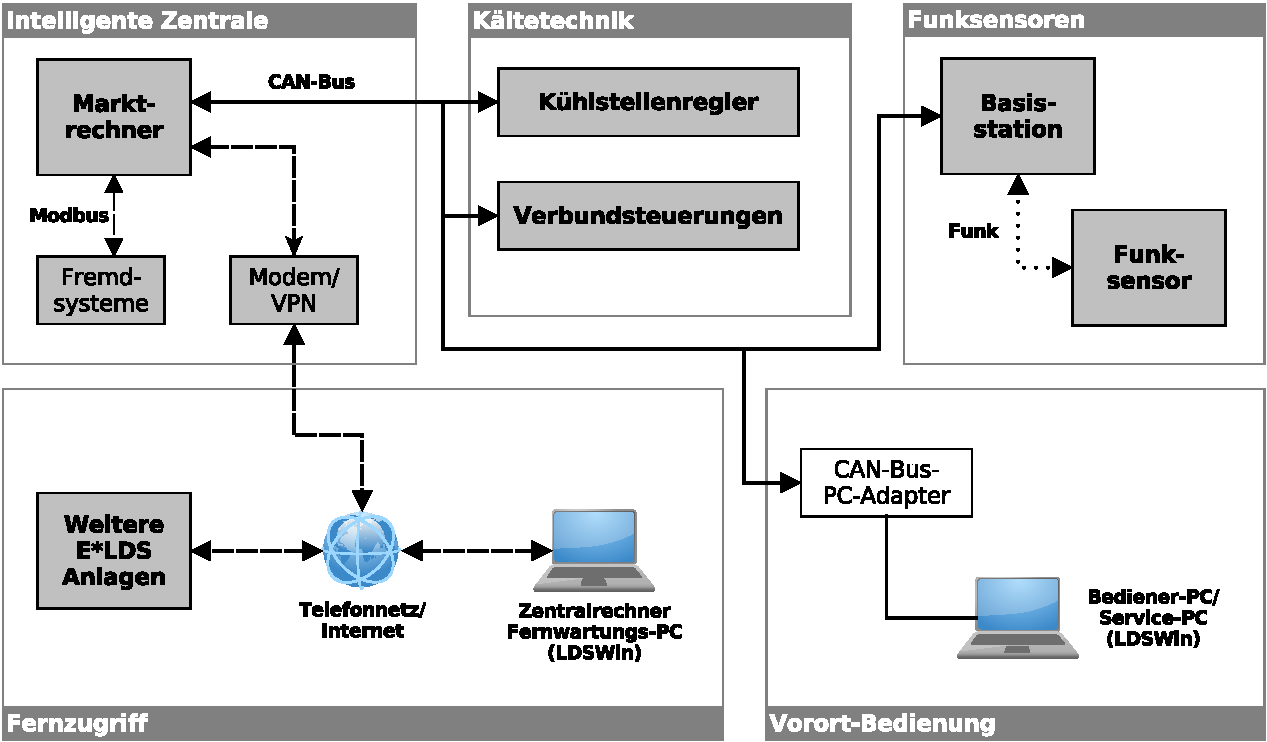
\includegraphics[scale=0.65]{images/kaelteanlage_uebersicht.pdf}
\caption{Übersicht einer Kälteanlage}
\label{fig:kaelteanlage}
\end{figure}

\subsection{Marktrechner} \label{sec:marktrechner} 
Betrachtet man eine Kälteanlage, dann ist der Marktrechner ihr Herzstück. Über den CAN-Bus ist er in der Lage, Komponenten zentral zu parametrieren und zu überwachen. Sämtliche Betriebsdaten und Betriebszustände, Meldungen und Alarme aus der Überwachung werden auf seinem internen Speicher archiviert \cite{elds}.

\paragraph{Hardware} Der Marktrechner verfügt über einen 32-Bit-Prozessor aus der ARM-Prozessorfamilie. Für die persistente Datenspeicherung steht eine fest verbaute zur Verfügung SD-Karte. Dazu gibt es 256-MB flüchtigen RAM-Speicher. Als Zentrale Komponente benötigt der Marktrechner einige Schnittstellen für die Kommunikation, diese sind in Abbildung~\ref{fig:marktrechner_interfaces} zu sehen. Über den Ethernet-Port ist der Marktrechner mit dem Unternehmensnetzwerk verbunden, darüber kann für die Fernwartung zugegriffen werden. Über die drei RS-232 COM-Schnittstellen kann ein PC vor Ort angeschlossen werden, die Fernwartung via Modem erfolgen, das M-Bus-Gateway zur Verbrauchsdatenerfassung verbunden werden oder Sonderfunktionen, beispielsweise Gebäudeleittechnik oder sonstige Fremdsysteme, bedient werden. Über die RS-485 COM-Schnittstelle können Modbus-Regler hinzugefügt werden. Die USB-Anschlüsse sind für zukünftige Benutzung vorgesehen. Einer der beiden CAN-Bus-Anschlüsse wird benutzt, um mit den E*LDS-Komponenten zu kommunizieren. Der zweite Anschluss ist für zukünftige Benutzung vorgesehen und über die zwei Digitaleingänge können entweder Alarme entgegengenommen oder Energiezähler ausgelesen werden. Die Benutzerinteraktion findet über ein 7-Zoll Touch-Display statt.

\begin{figure}[htbp]
\centering
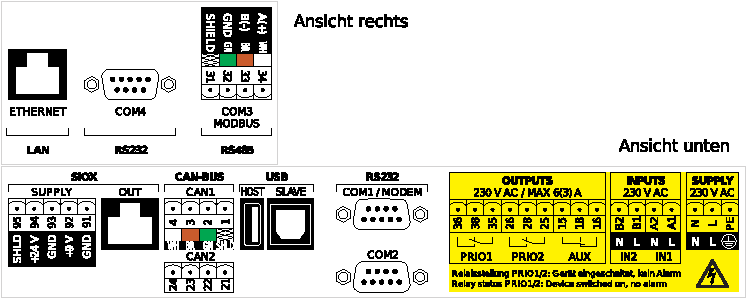
\includegraphics[scale=1.1]{images/CI4000_Hardware_Sticker.pdf}
\caption{Schnittstellen des Marktrechners}
\label{fig:marktrechner_interfaces}
\end{figure}

\paragraph{Software}

Das Betriebssystem auf dem Marktrechner ist eine eigene Linux-Distribu\-tion, welche mit der Software ptxdist der Pengutronix e.K. erstellt wird. Ptxdist bringt einige hundert Module und Bibliotheken mit. Darunter sind etwa, der leichtgewichtige HTTP-Server lighttpd, der SSH-Server openssh oder das Synchronisierungstool rsync. Mit ein wenig Konfigurationsaufwand können auch eigene Module hinzugefügt werden. Über eine Toolchain, die ebenfalls von der Pengutronix e.K. geliefert wird, kann eine sehr schlanke Distribution, für viele Prozessorarchitekturen,  erzeugt werden, die auf den eigenen Software-Stack zugeschnitten ist. Die eigenen Softwaremodule sind in C++ und mit dem Qt-Framework geschrieben. 

\paragraph{Funktionen} \label{para:architektur}

Alle Daten und Meldungen, die der Marktrechner sammelt und aufbereitet müssen ausgewertet werden. Die 24-Stunden Überwachung vor Ort, durch einen Mitarbeiter des Eigentümers, ist nicht wirtschaftlich. Auch das Fachliche Wissen zur Betreuung einer Kälteanlage ist beim Endkunden nicht vorhanden. Deshalb übernehmen heutzutage großteils Fernservice-Zentralen (FSZs) die Überwachung von Kälteanlagen. FSZs haben in der Kältetechnik ausgebildete Mitarbeiter, die Daten und Meldungen des Marktrechners verstehen können. Der Marktrechner kann aus der Ferne über eine Ethernet- oder Modem-Verbindung erreicht werden. Letztere wird, aufgrund ihres aussterbendes Charakters, an dieser Stelle nicht weiter erläutert. Für den Zugriff auf die Ethernet-Schnittstelle sind Fernservice-Zentralen über VPN mit einem oder mehreren Unternehmensnetzwerken ihrer Kunden verbunden (Abbildung~\ref{fig:current_setup}). Über dieses können die Marktrechner erreicht werden. Auf diese Weise kann eine einzige Fernservice-Zentrale Tausende Marktrechner überwachen. Der Marktrechner fungiert als Server, das heißt, Daten und Meldungen müssen aktiv von einer Fernservice-Zentrale abgeholt werden. Ist aus den abgeholten Daten ersichtlich, dass ein Fehler in der Anlage aufgetreten ist, kann die Fernservice-Zentrale entweder direkt eingreifen oder einen Monteur zum betreffenden Kunden schicken, der die Anlage instand setzt.

\begin{comment}
@startuml images/problemfeld.svg
skinparam monochrome true
skinparam dpi 150

package "Unternehmensnetzwerk A" as UA {
  [Marktrechner 1]
  [Marktrechner 2]
  [...]
  [Marktrechner n]
}

package "Unternehmensnetzwerk B" as UB {
}

package "Unternehmensnetzwerk C" as UC {
}

cloud VPN {
}

[Fernservice-Zentrale] -down- VPN
VPN -down- UA
VPN -left- UB
VPN -right- UC
UA - [Marktrechner n]
UA - [...]
UA - [Marktrechner 2]
UA - [Marktrechner 1]

@enduml
\end{comment}

\begin{figure}[htbp]
\centering
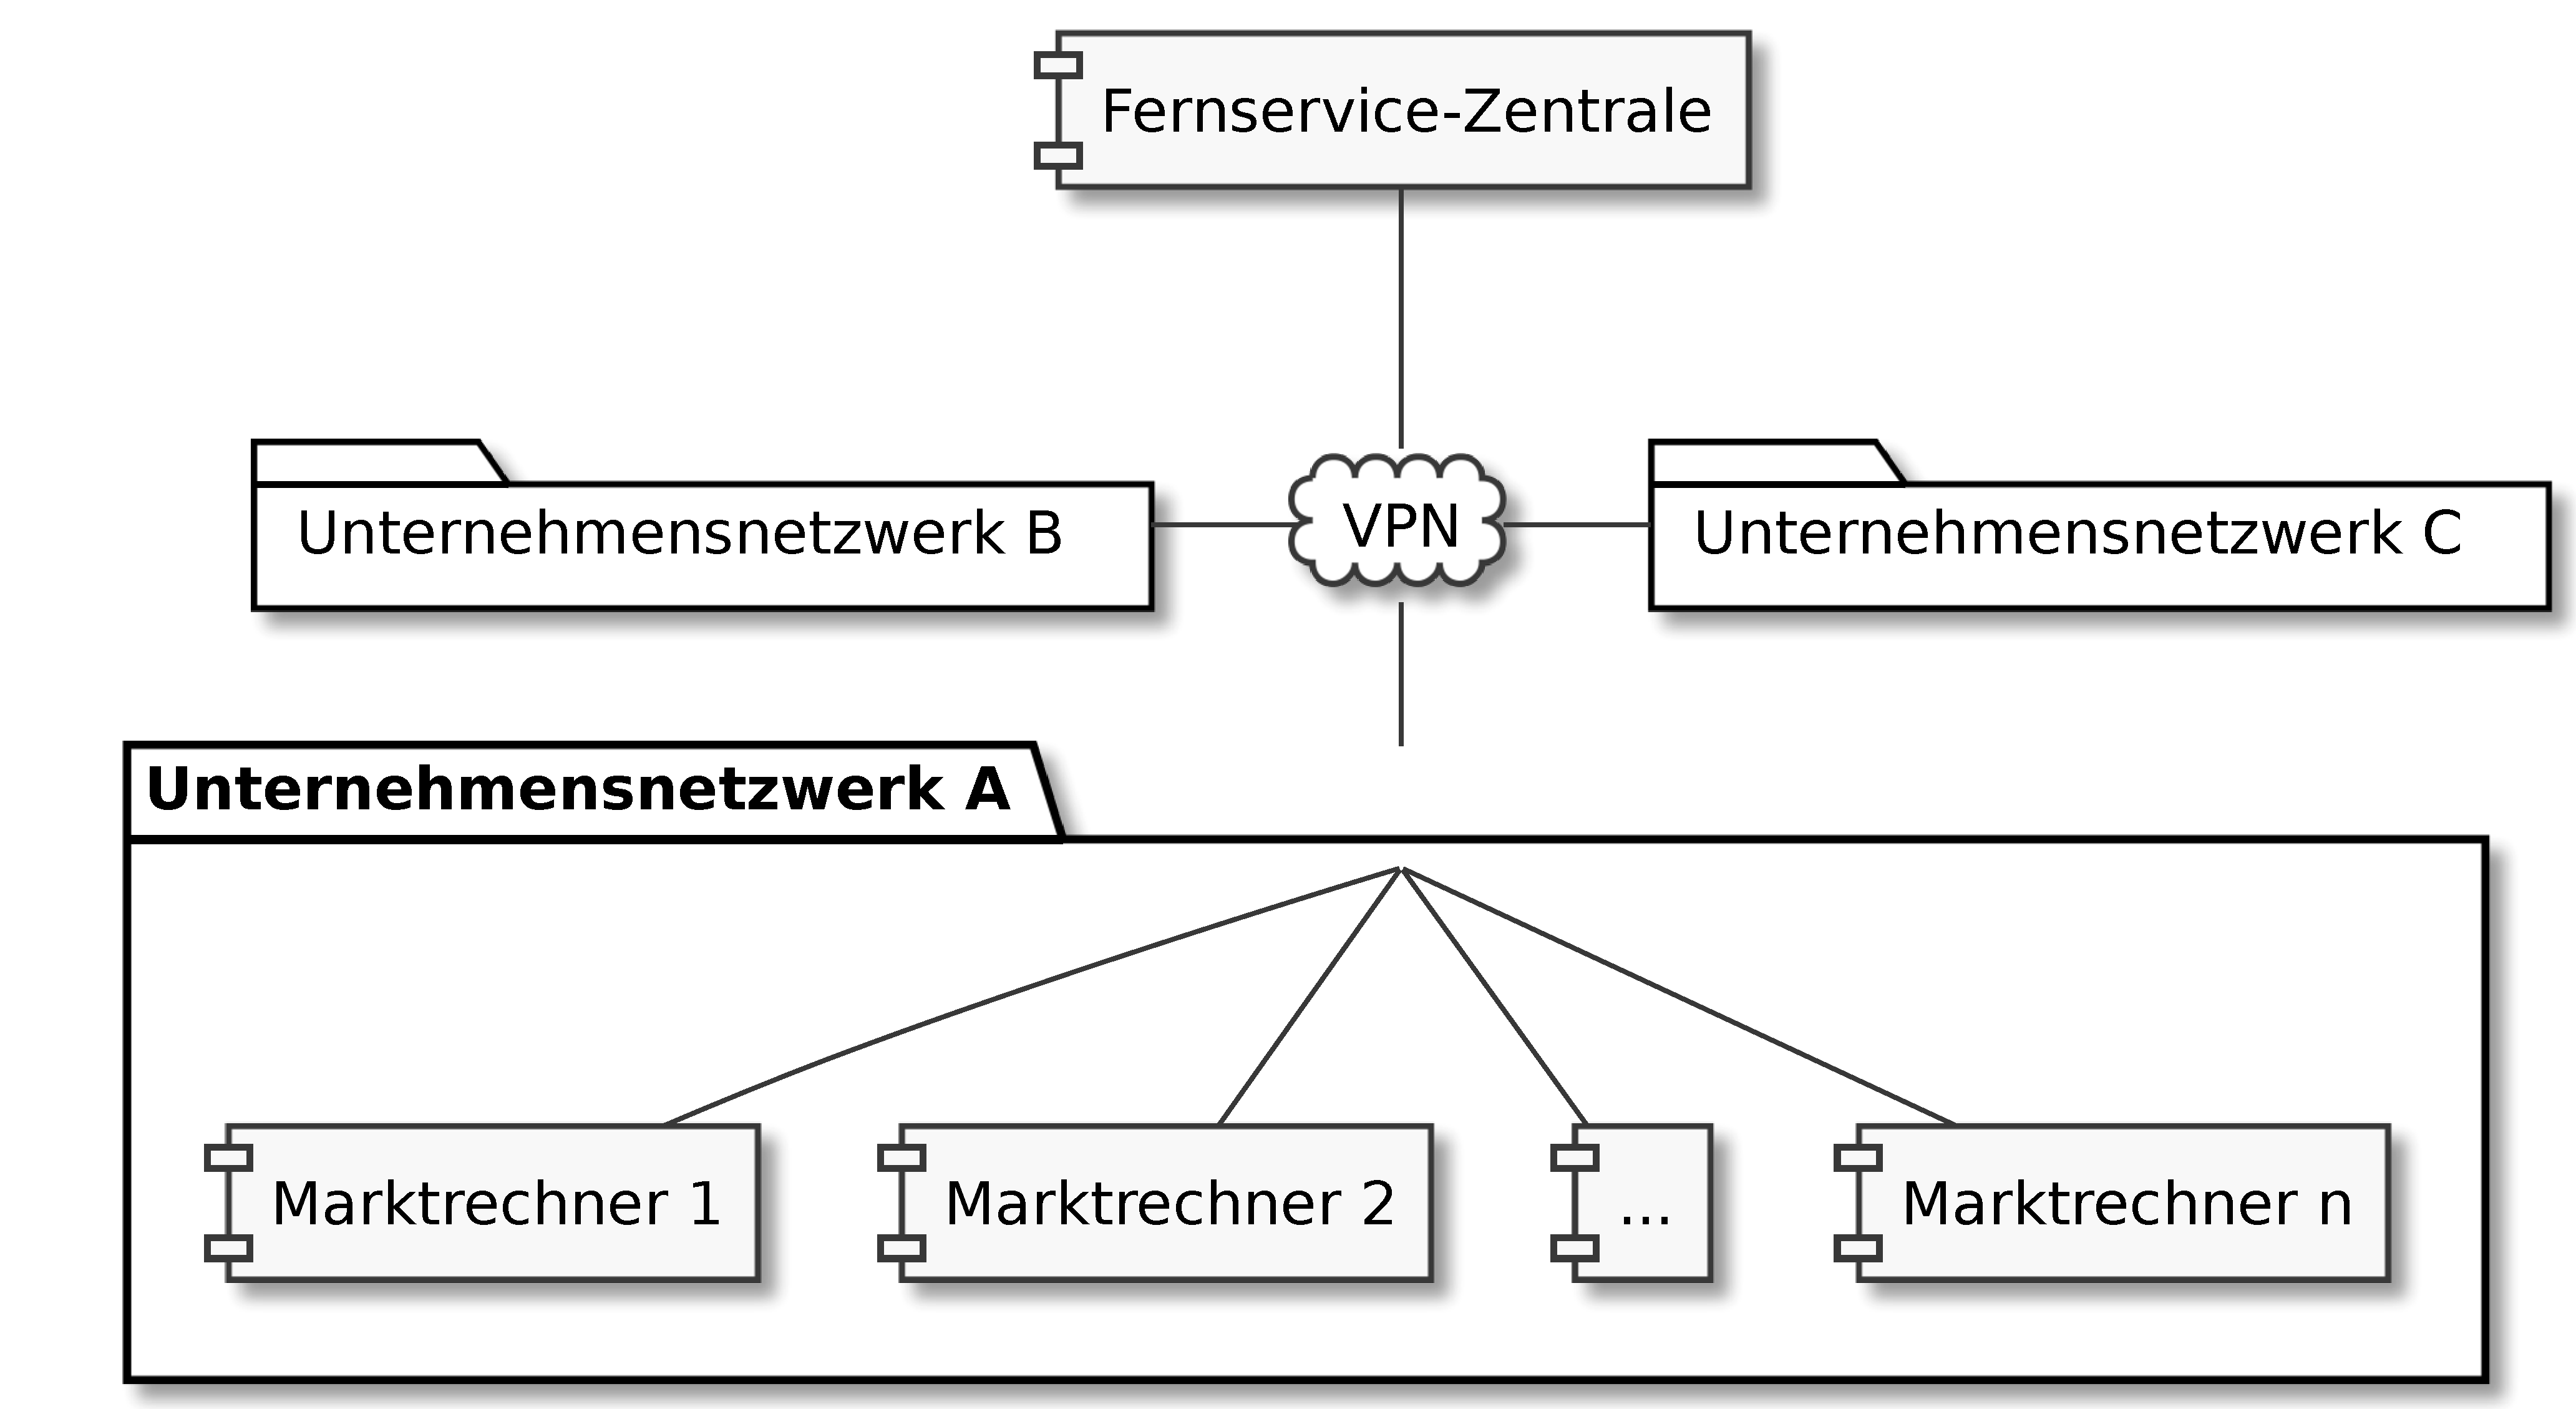
\includegraphics[scale=0.19]{images/problemfeld.pdf}
\caption{Aktuelle Architektur}
\label{fig:current_setup}
\end{figure}

Beim Einsatz von VPN ist die Kommunikation von der Fernservice-Zentrale bis zum Unternehmensnetzwerk abgesichert. Im Lokal Area Network (LAN) des Unternehmens ist der gesamte Datenverkehr zu und von den Marktrechnern allerdings unverschlüsselt. Aktuell gibt es zwei Arten von Datenverkehr zwischen Marktrechner und FSZ, zum einen über das proprietäre Protokoll des Herstellers und zum anderen über Webservices auf Basis von einfachen XML-RPCs.

--> nach Analyse verschieben

Ein Angreifer mit Zugriff auf das LAN und Kenntnisse des Hersteller-Protokolls hätte die Möglichkeit, den Datenverkehr zwischen Fernservice-Zentrale und Marktrechner mitzulesen. Viel schwerwiegender als das Mitlesen der Kommunikation ist, dass ein solcher Angreifer über das Protokoll vollen lesenden und schreibenden Zugriff, auf das System erhalten kann, da es keine geeignete Autorisierung und Authentifizierung gibt. Die Anzahl an Personen mit Wissen über das Hersteller-Protokoll schränkt allerdings den Kreis der möglichen Angreifer ein. Viel wahrscheinlicher ist ein Angreifer mit Zugriff auf das LAN ohne Kenntnisse des Hersteller-Protokolls. Dieser kann den Datenverkehr zwischen XML-RPC und Fernservice-Zentrale mithören. Da in der XML die Daten interpretierbar aufbereitet wurden, ist es ein Leichtes, diese Daten auszuwerten. Auch hier sind keine geeignete Autorisierungs- und Authentifizierungstechniken eingesetzt, wodurch der Angreifer statt mitzulesen, den XML-RPC selbst befragen könnte. Dadurch erlangt er zwar keine vollen Zugriff auf das System, kann jedoch einige wichtige Schnittstellen auslesen und zum Teil auch neu konfigurieren. 

Eine weitere Schwachstelle ist, dass der Hersteller durch die existierende End-to-Site VPN-Verbindung keinen Zugriff auf die Systeme erlangen kann, um Unterstützung bei Problemen zu leisten. Die VPN-Architektur erfüllt zwar alle Anforderungen an die Sicherheit, schränkt jedoch den Anwendungsbereich in heutigen verteilten Systemen stark ein.

\subsection{RestGateway} 

Das RestGateway ist die Neuauflage des XML-RPC. Es wurde, vom Author dieser Thesis, im Rahmen des vor der Thesis absolvierten Praktikums entwickelt. Es basiert auf dem Representational State Transfer (REST) Konzept zur Entwicklung von Webanwendungen. REST ist keine explizite Norm, sondern bezeichnet vielmehr die Idee, dass eine URL genau einen Seiteninhalt als Ergebnis einer serverseitigen Aktion liefert \cite{wiki_rest}. REST nutzt Standard HTTP-Befehle, um lesend und schreibend auf Ressourcen zuzugreifen. Zur Zeit sind ausschließlich lesende Zugriffe implementiert, welche über URLs abgerufen werden können. Diese Aufrufe liefern interpretierte Inhalte im XML oder JSON Format. Zudem gibt es eine generische Schnittstelle, welche als Proxy für CAN-Nachrichten fungiert, dadurch können beliebige CAN-Nachrichten über HTTP/S gesendet werden, auch solche, die schreibend auf das System zugreifen. Das RestGateway bietet keinerlei Mechanismus für die Authentifizierung und Autorisierung. Eine Erweiterung wäre auf Basis dieser Arbeit denkbar. Das RestGateway kann in zwei Ausführungen installiert werden, entweder als Modul auf dem Marktrechner (Abbildung~\ref{fig:rest_intern}), wo es den XML-RPC ersetzt, oder auf einem externen Server (Abbildung~\ref{fig:rest_extern}), wo es Anfragen an mehrere Marktrechner senden kann. Die unterschiedlichen Ausführungen werden durch das LanGateway-Modul des Marktrechners ermöglicht. Diese ist eine TCP-Schnittstelle, welche als Proxy zwischen TCP-Netzwerk und CAN-Netzwerk fungiert. Über TCP werden die CAN-Nachrichten, ohne Daten-Wrapper wie XML, als Bytestrom übertragen.

\begin{figure}[htbp]
\centering
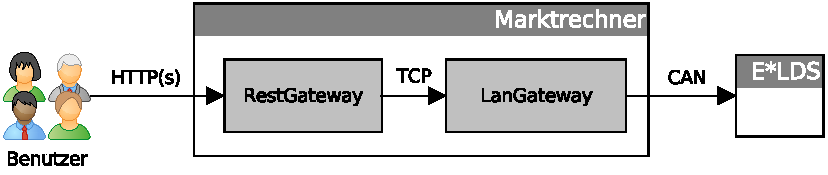
\includegraphics[scale=0.7]{images/RestGateway_intern.pdf}
\caption[]{RestGateway als Marktrechner-Modul}
\label{fig:rest_intern}
\end{figure}

Intern ist das RestGateway ein Wrapper über dem LanGateway, welches interpretierte Inhalte in einem menschenlesbaren Format liefert.

\begin{figure}[htbp]
\centering
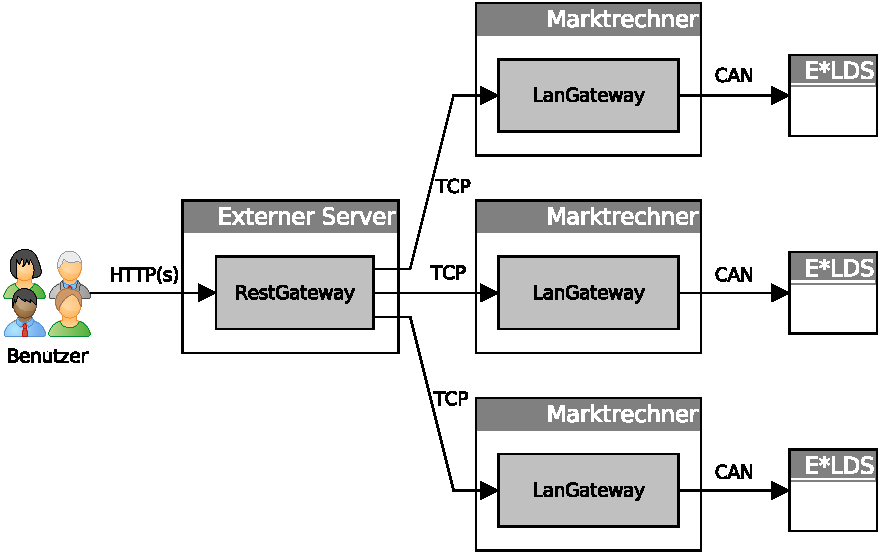
\includegraphics[scale=0.7]{images/RestGateway_extern.pdf}
\caption[]{RestGateway auf externen Server}
\label{fig:rest_extern}
\end{figure}

Extern bietet das RestGateway die Möglichkeit, über die REST-Schnittstellen verschiedene Marktrechner abzufragen. Dieses Feature ist vor allen Dingen für Fernservice-Zentralen interessant, da dort viele Marktrechner verwaltet werden (vgl. \ref{para:architektur}). Des Weiteren können über diesen Weg neue Funktionen ohne große Testvorbereitungen erprobt werden, denn es wird kein aufwendiges Update der Marktrechner-Software notwendig. Ein solches Update ist deshalb so Aufwendig, da es beim Endkunden erfolgen muss, weil aufgrund der Kosten, weder Hersteller noch Fernservice-Zentralen, eine Kälteanlage zu Testzwecken betreiben und zum anderen werden bei einem Update zwangsläufig auch andere Software-Module upgedatet, wodurch ein solche Update großer Vorbereitung bedarf.

\subsection{Alarmmanagement} 

Das Alarmmanagement beschreibt die Reaktion auf Fehlfunktionen einer Kälteanlage. Jede Kälteanlage ist anders und nutzt unterschiedliche Kühlmöbel, deshalb müssen Alarme speziell konfiguriert werden. Ein Alarm trifft eine Aussage über den Betriebszustand der Kälteanlage, beispielsweise soll ein Alarm ausgelöst werden, wenn die Temperatur in einem Kühlmöbel einen bestimmten Grenzwert überschreitet beziehungsweise unterschreitet. Damit auf Alarme reagiert werden kann, werden Anlagen überwacht. Dazu können Alarme entweder von Fernwarten in bestimmten Intervallen, etwa alle 15 Minuten, ausgelesen werden, oder alternativ können Alarme durch das System selbstständig per E-Mail- oder per SMS-Benachrichtigung versenden. Zusätzlich ist im Marktrechner eine Hupe installiert, die auf Fehlfunktionen vor Ort aufmerksam macht. 

\subsection{Offline-Konfiguration} 

Eine Offline-Konfiguration ist eine an den Markt angepasste Konfiguration der Kälteanlage, welche vor Inbetriebnahme erstellt wurde. Ein Teil ist unter anderem die genaue Parametrierung der Kühlgeräte und Kühlmöbel, unter Berücksichtigung der darin zu lagernden Waren. Ein weiterer Teil der Offline-Konfiguration sind auch die Alarme. Die technischen Konfiguration des Marktrechners, beispielsweise Netzwerkkonnektivität, Internetzugang oder Berechtigungsnachweise, sind aktuell nicht in der Offline-Konfiguration enthalten.

\section{Sicherheit} \label{sec:security_conzept}

Viele Sicherheitssysteme heutzutage sind \textit{"sicher"}, da sich niemand die Mühe gemacht hat, diese anzugreifen \cite[s.~0]{gutmann}. Ein Großteil der Problemen von Sicherheitskonzepten entsteht, weil die Anforderungen an Sicherheit erst im Nachhinein aufkommen, wenn das eigentliche System schon fertig konzipiert oder implementiert ist. Meist wird dann versucht, die Sicherheit irgendwie noch an das System anzuheften. Sicherheit wirkt in diesen Fällen oft wie ein fünftes Rad am Wagen, wodurch Systeme entstehen, die für den Anwender extrem mühselig zu benutzen sind. Dabei sollte berücksichtigt werden, dass Benutzer Sicherheit lieber ausschalten oder umgehen als sich damit auseinanderzusetzen \cite[s.~5]{gutmann}. Bevor man über potentielle Eigenschaften eines Sicherheitssystems nachdenkt, sollte man daher zunächst das Umfeld betrachten, in welchem das System eingesetzt werden soll \cite[s.~4]{gutmann}. Wenn heutzutage über Sicherheit diskutiert wird, wird meistens ausschließlich über Kryptographie gesprochen. Auch wenn Kryptographie Hauptbestandteil jedes Sicherheitssystems ist, ignorieren praktisch alle Angriffe auf ein Sicherheitssystem die Kryptographie und attackieren den Weg wie diese genutzt wird \cite[s.~1]{gutmann}. Ein bekanntes Beispiel ist der Heartbleed-Bug\footnote{(Q2/2014) weitere Informationen unter http://heartbleed.com}, der eine Lücke in der Heartbeat-Implementierung, der OpenSSL Bibliothek, ausnutzt, um sich Zugriff auf den Privaten Kommunikationsschlüssel zu verschaffen. Es macht also wenig Sinn die Kryptographischen Mittel auszureizen, wenn kein Angreifer diese versucht zu attackieren. Zudem wird durch Verschlüsselung das Hauptproblem eines Sicherheitssystems, nämlich \textit{"Vertrauen"}, nur unzureichend betrachtet. Das Problem, die Authentifizierung effizient und zuverlässig über einen einzigen Kommunikationskanal zu lösen besteht bis heute, ohne das es eine etablierte Lösung dafür gibt (vgl.~\ref{sec:auth_modells}). 

Teil des Sicherheitskonzeptes dieser Arbeit wird es sein, dieses Authentifizierungsproblem auf geeignete Weise zu berücksichtigen, ohne dass durch den Einsatz einer bestimmten Technologie im Extremfall enorme Kosten entstehen können. Ein solcher Extremfall würde eintreten, wenn durch die Kompromittierung der Software oder Hardware alle Berechtigungsnachweise manuelle ausgetauscht werden müssen.

\subsection{Sicherheitsstandards} \label{sec:sec_standard}

Sicherheitsstandards sind von Staaten festgelegte Anforderungen an sichere Systeme. Die Standards klassifizieren sichere Systeme anhand von Stufen, je höher die Stufe, desto mehr Aufwand ist nötig, um diesen zu erreichen. Der erste Sicherheitsstandard mit hohem Verbreitungsgrad war der Trusted Computer System Evaluation Criteria (TCSEC) und wurde 1983 vom amerikanischen Department of Defense (DOD) veröffentlicht. Vor 1990 veröffentlichten auch andere Regierungen, unter anderen Kanada, Westdeutschland, Frankreich und Großbritannien eigene Standards. Da diese Standards nur in den jeweiligen Ländern verwendet wurden und es keine internationale Anerkennung gab, hat die EU 1990 den Standard Information Technology Security Evaluation Criteria (ITSEC) für Europäische Staaten veröffentlicht. Dieser Standard war jedoch auf Europa begrenzt, weshalb 1996, mit den Common Criteria (CC), ein weltweit anerkannt Standard gebildet wurde. Beteiligte Staaten an den CC sind Australien/Neuseeland, Kanada, Frankreich, Deutschland, Japan, Niederlande, Spanien, Großbritannien und die USA.

\subsubsection{Common Criteria}

Die Common Criteria sieht sieben Sicherheitsstufen für die Klassifizierung vor. Diese Evaluation Assurance Level (EAL) sind bis Stufe 4 international anerkannt. Der Aufwand, der für höhere Stufen betrieben werden muss, ist so umfangreich, dass er nur für eine Minderheit an Unternehmen in Frage kommt. Die aktuelle Version 3.1. Release 4 wurde im September 2012 veröffentlicht. Alle weiteren Erläuterungen beziehen sich auf diese Version und sind den Quellen \cite{ccp1, ccp2, ccp3, bsi_ccguide} entnommen.

\paragraph{Klassifizierung}

Die sieben EAL-Stufen haben Anforderungen in sechs Assurance-Klassen, wobei eine Assurance-Klasse aus mindestens einer Assurance-Familie besteht (Abbildung~\ref{fig:eal_sum}). Die Familien sind dabei selbst in Stufen eingeteilt. Die Anzahl der Stufen in den Familien ist von Familie zu Familie unterschiedlich. Beispielsweise fordert EAL-3 aus der Klasse "Tests" in der Familie "Analyse der Abdeckung" (ATE\_COV) die Stufe 2 und aus der Klasse "Entwicklung" in der Familie "Funktionale Spezifikation mit kompletter Zusammenfassung" (ADV\_FSP) die Stufe 3. Einige Familien sind erst ab höheren EAL Stufe erforderlich oder sind komplett optional. 

\begin{figure}[htbp]
\centering
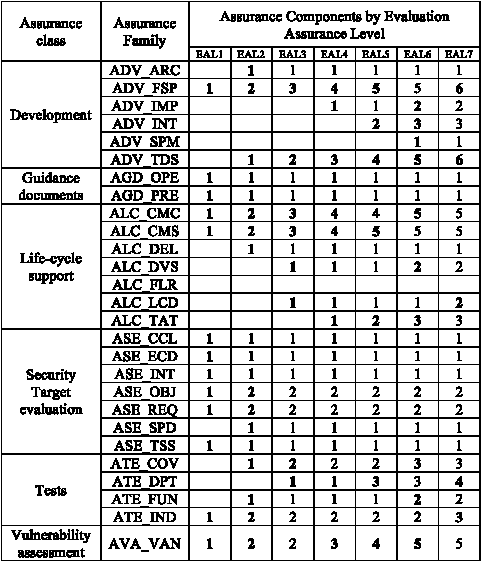
\includegraphics[scale=1]{images/cc_eal_table.pdf}
\caption[]{Evaluation assurance level Zusammenfassung aus \cite{bsi_ccguide}}
\label{fig:eal_sum}
\end{figure}

\paragraph{Vorgehen}

Für die Zertifizierung sieht die Common Criteria zwei Möglichkeiten vor. Zum einen kundengetrieben, zum anderen entwicklergetrieben. Bei der ersten Möglichkeit stellt der Kunde seine Anforderungen an Hardware und Software in einem Protection Profile (PP) zusammen. Anhand dessen kann er das im PP beschriebene System oder Produkt in Auftrag geben. Alternativ kann er anhand dessen existierende Lösungen evaluieren. Die Entwickler müssen mit dem Security Target (ST) nachweisen, dass das entwickelte System/Produkt den Anforderungen aus dem Protection Profile genügt. Mit Hilfe von PP und ST kann von einer unabhängigen Prüfstelle zertifiziert werden, dass die Inhalte und die Umsetzung der beiden Dokumente der Wahrheit entsprechen.

\begin{figure}[htbp]
\centering
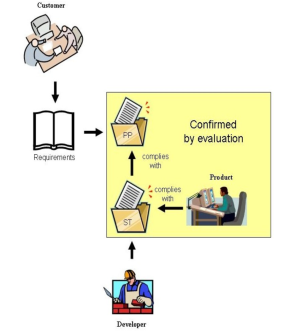
\includegraphics[scale=1.3]{images/cc_prozess.pdf}
\caption[]{Common Criteria Vorgehen aus \cite{bsi_ccguide}}
\label{fig:cc_prozess}
\end{figure}

Die Inhalte aus Protection Profile und Security Target sind großteils identisch, wobei das ST zusätzlich die technische Umsetzung beschreiben muss. Bei der zweiten Möglichkeit fällt der Kunden weg und die Entwickler schreiben ein Security Target, um von einer Prüfstelle ein Zertifikat zu erhalten, welches als Qualitätsmerkmal ihres Produktes beworben werden kann. Im Rahmen dieser Thesis sind die expliziten Inhalte des ST nicht von Interesse.

\paragraph{Protection Profile}

Die Erstellung eines Protection Profiles, wird im Folgenden mit der Erklärungs-Methode beschrieben, welche aus aus insgesamt sechs Teilen besteht. Das Vorgehen dieser Methode soll vor allen Dingen Verständlichkeit beim Leser schaffen. Die Informationen darüber stammen aus \cite{bsi_ccguide}.
\begin{enumerate}
\item Als erstes werden Konformitätsansprüche beschrieben. Darunter fallen Verweise auf die Version des CC, abhängige Protection Profile und welche EAL-Pakete genutzt werden. Abschließend wird noch beschrieben, wie strikt sich PPs und STs, die diese PP benutzen wollen an die Inhalte halten müssen.
\item Im zweiten Schritt werden die Sicherheitsprobleme definiert. Dabei werden in Bezug auf das zu evaluierende Ziel (Target of Evaluation--TOE) Gesetze, sonstige Regulierungen und Bedrohungen analysiert. Bei den Bedrohungen liegt der Fokus auf den zu schützenden Gütern.
\item Im dritten Schritt werden zu den Sicherheitsproblemen, aus den vorherigen Schritt, abstrakte, präzise Lösungsvorschläge erarbeitet. Dabei soll sich auf das "Was" konzentriert werden und nicht beschrieben werden "Wie" etwas zu lösen ist. Im CC-Kontext hießen diese Lösungsvorschläge Security Objects. 
\item Im vierten Schritt wird für jedes Security-Object ein detailliertes Security Functional Requirement (SFR) erfasst. Die SFRs werden dabei an relevante, thematische Gruppen gekoppelt, welche im CC-Standard vorgegeben sind. Die Beschreibung als SFR umfasst die Beteiligten, die Informationsflüsse, die Operationen und die Daten. Mit Abschluss dieses Schrittes sind die Sicherheitsanforderungen an das System beziehungsweise Produkt festgelegt. 
\item Im Schritt fünf werden Security Assurance Requirements (SAR) festgelegt. Diese sagen aus, wie das TOE zu evaluieren ist und ermöglichen dadurch den Vergleich von zwei Security Targets.
\item Die Einleitung kommt zum Schluss, sie fasst die Inhalte des PP in Prosa zusammen und führt den Leser in die Thematik ein.
\end{enumerate}

\subsection{Sicherheitsmodell}

Ein Sicherheitsmodell bietet einen Leitfaden zur Erstellung eines Sicherheitskonzeptes. Ein ganzheitliches Modell stellt das Bundesamt für Sicherheit in der Informationstechnik (BSI) in seinem IT-Grund\-schutz.

\subsubsection{BSI Sicherheitsmodell}

Folgende Ausführungen sind dem BSI IT-Grundschutzempfehlungen entnommen \cite{bsi_grundsch1,bsi_grundsch2,bsi_grundsch3,bsi_grundsch4}.
Das Ziel des Grundschutzes ist das Erreichen eines mittleren, angemessenen und ausreichenden Schutzniveaus für IT-Systeme \cite{wiki_itgrundschutz}. Zu diesem Zweck stellt das BSI ein Modell, zur Entwicklung von Sicherheitskonzepten, zur Verfügung. In Abbildung~\ref{fig:bsi_sicherheit} sind die empfohlenen Schritte gezeigt. Schritt eins verlangt die Erfassung aller Komponenten im Geltungsbereich. Dazu soll das Zusammenspiel zwischen Geschäftsprozessen und Anwendungen herausgearbeitet werden. Als nächstes soll der Schutzbedarf der Komponenten aus Schritt eins ermittelt werden. Der ermittelte Schutz soll gemäß der eingesetzten Informationstechnik ausreichend beziehungsweise angemessen sein. Anhand dieser Informationen werden für die Zielobjekte aus Strukturanalyse und Schutzbedarf Bausteine aus dem IT-Grundschutz gewählt. Der anschließende Basis-Sicherheitscheck soll das aktuelle Sicherheitsniveau einschätzen und liefert als Ergebnis eine Liste der relevanten Maßnahmen und ihren Umsetzungsstatus "entbehrlich", "ja", "teilweise" oder "nein". Dafür sollen Gefährdungenkataloge und Maßnahmenkataloge des BSI genutzt werden. In Schritt vier wird geprüft, ob die Standard-Sicherheitsmaßnahmen ausreichend sind, was für die meisten typischen Geschäftsfelder der Fall sein sollte. Sollten erweitere Sicherheitsmaßnahmen nötig werden, muss für diese eine Risikoanylse durchgeführt werden. Bei den Standard-Sicherheitsmaßnahmen ist dies bereits durch die IT-Grundschutz-Kataloge abgedeckt. 
\begin{figure}[htbp]
\centering
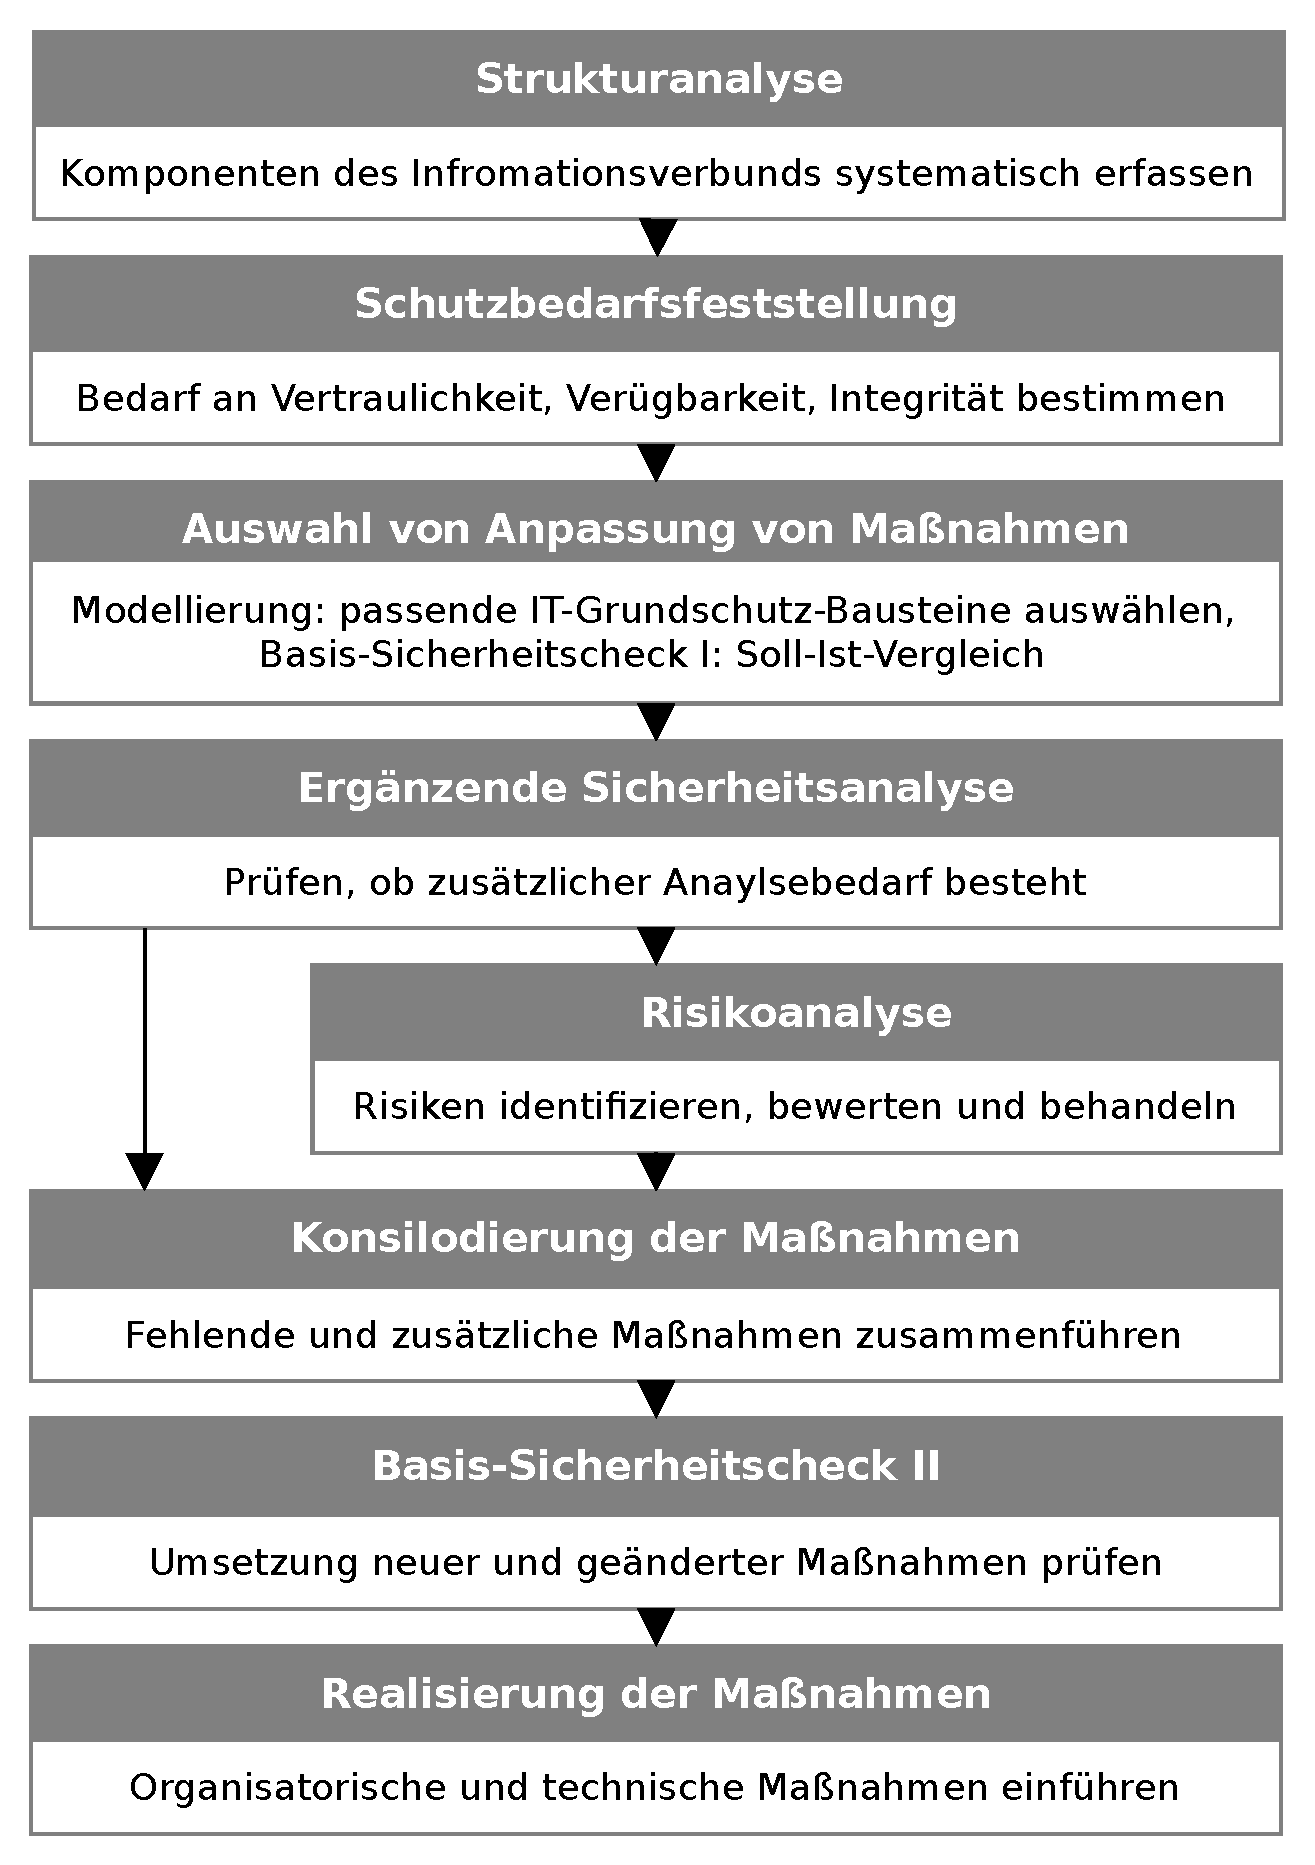
\includegraphics[scale=0.7]{images/bsi_sicherheitskonzept.pdf}
\caption[BSI Sicherheitskonzept]{BSI Sicherheitskonzept\footnotemark}
\label{fig:bsi_sicherheit}
\end{figure}
Ab Schritt sechs erfolgt die Durchführung der Maßnahmen. Bei der Konsolidierung wird geprüft, welche Maßnahmen aus den IT-Grundschutz-Katalogen tatsächlich in der Praxis umsetzbar sind. Teilweise müssen einige Maßnahmen noch an Gegebenheiten im Unternehmen angepasst werden. Unter Berücksichtigung des verfügbaren Budgets und des verfügbaren Personals werden die entsprechenden Maßnahmen für die Umsetzung geplant. Im zweiten Sicherheitscheck wird abschließend ein erneuter Soll-Ist-Vergleich durchgeführt, um die Ergebnisse der Maßnahmen zu überprüfen. Als letzter Schritt werden die Maßnahmen im Alltagsgeschäft in Betrieb genommen.
\footnotetext{Der Zeichnung \cite{bsi_img} des BSI nachempfunden, aufgrund unangemessener Bildqualität}

Das vom BSI vorgeschlagene Konzept und das damit verbundene Vorgehen betrachtet ein Sicherheitsmodell ausgiebig aus technischer Sicht. Es wurde entwickelt, um als internationaler Standard genutzt zu werden, dort hat es jedoch aufgrund schlechter englischer Übersetzung, keinerlei Verbreitung und auch in Deutschland ist die Verbreitung nur sehr gering \cite{bsi_kritik}. 

\subsection{Methoden zur Bedrohungsanalyse}

Zusätzlich zum Vorgehen des BSI werden weitere Methoden für die Bedrohungsanalyse vorgestellt, die nützlich für das Erstellen eines Sicherheitskonzept sind. Den Aufgrund von Finanznöten des BSI kann sich nicht darauf verlassen werden, dass die Inhalte des IT-Grund\-schutzes immer aktuell sind \cite{bsi_not}.

\subsubsection{Soft Systems Methodology} \label{sec:ssm}

Nachfolgende Erläuterungen beziehen sind auf \cite[s.~252]{gutmann}. 
Das Lösen von Sicherheitsproblemen ist ein kniffeliges Unterfangen, da die typische Vorgehensweise von vielen Informatikern, ein Problem mit Technologien zu bewerfen, nicht funktioniert. Fragt man diese--"Wie löst man das Problem, Benutzer sicher über das Internet zu authentifizieren?"--dann werden Antworten wie OpenID, LDAP, SecurID oder ähnliches zu hören sein. Nur die wenigsten werden fragen--"Wer soll, wo, wogegen authentifiziert werden, wie benutzerfreundlich (einfach) kann der Mechanismus sein und welches Budget steht zur Verfügung?"--Um das natürliche Verlangen, die Lieblingstechnologie verwenden zu wollen, zu unterdrücken, ist es sinnvoll, Problem Structuring Methods (PSK) einzusetzen. Eine dieser PSK-Methoden ist die Soft Systems Methodology (SSM).

\begin{figure}[htbp]
\centering
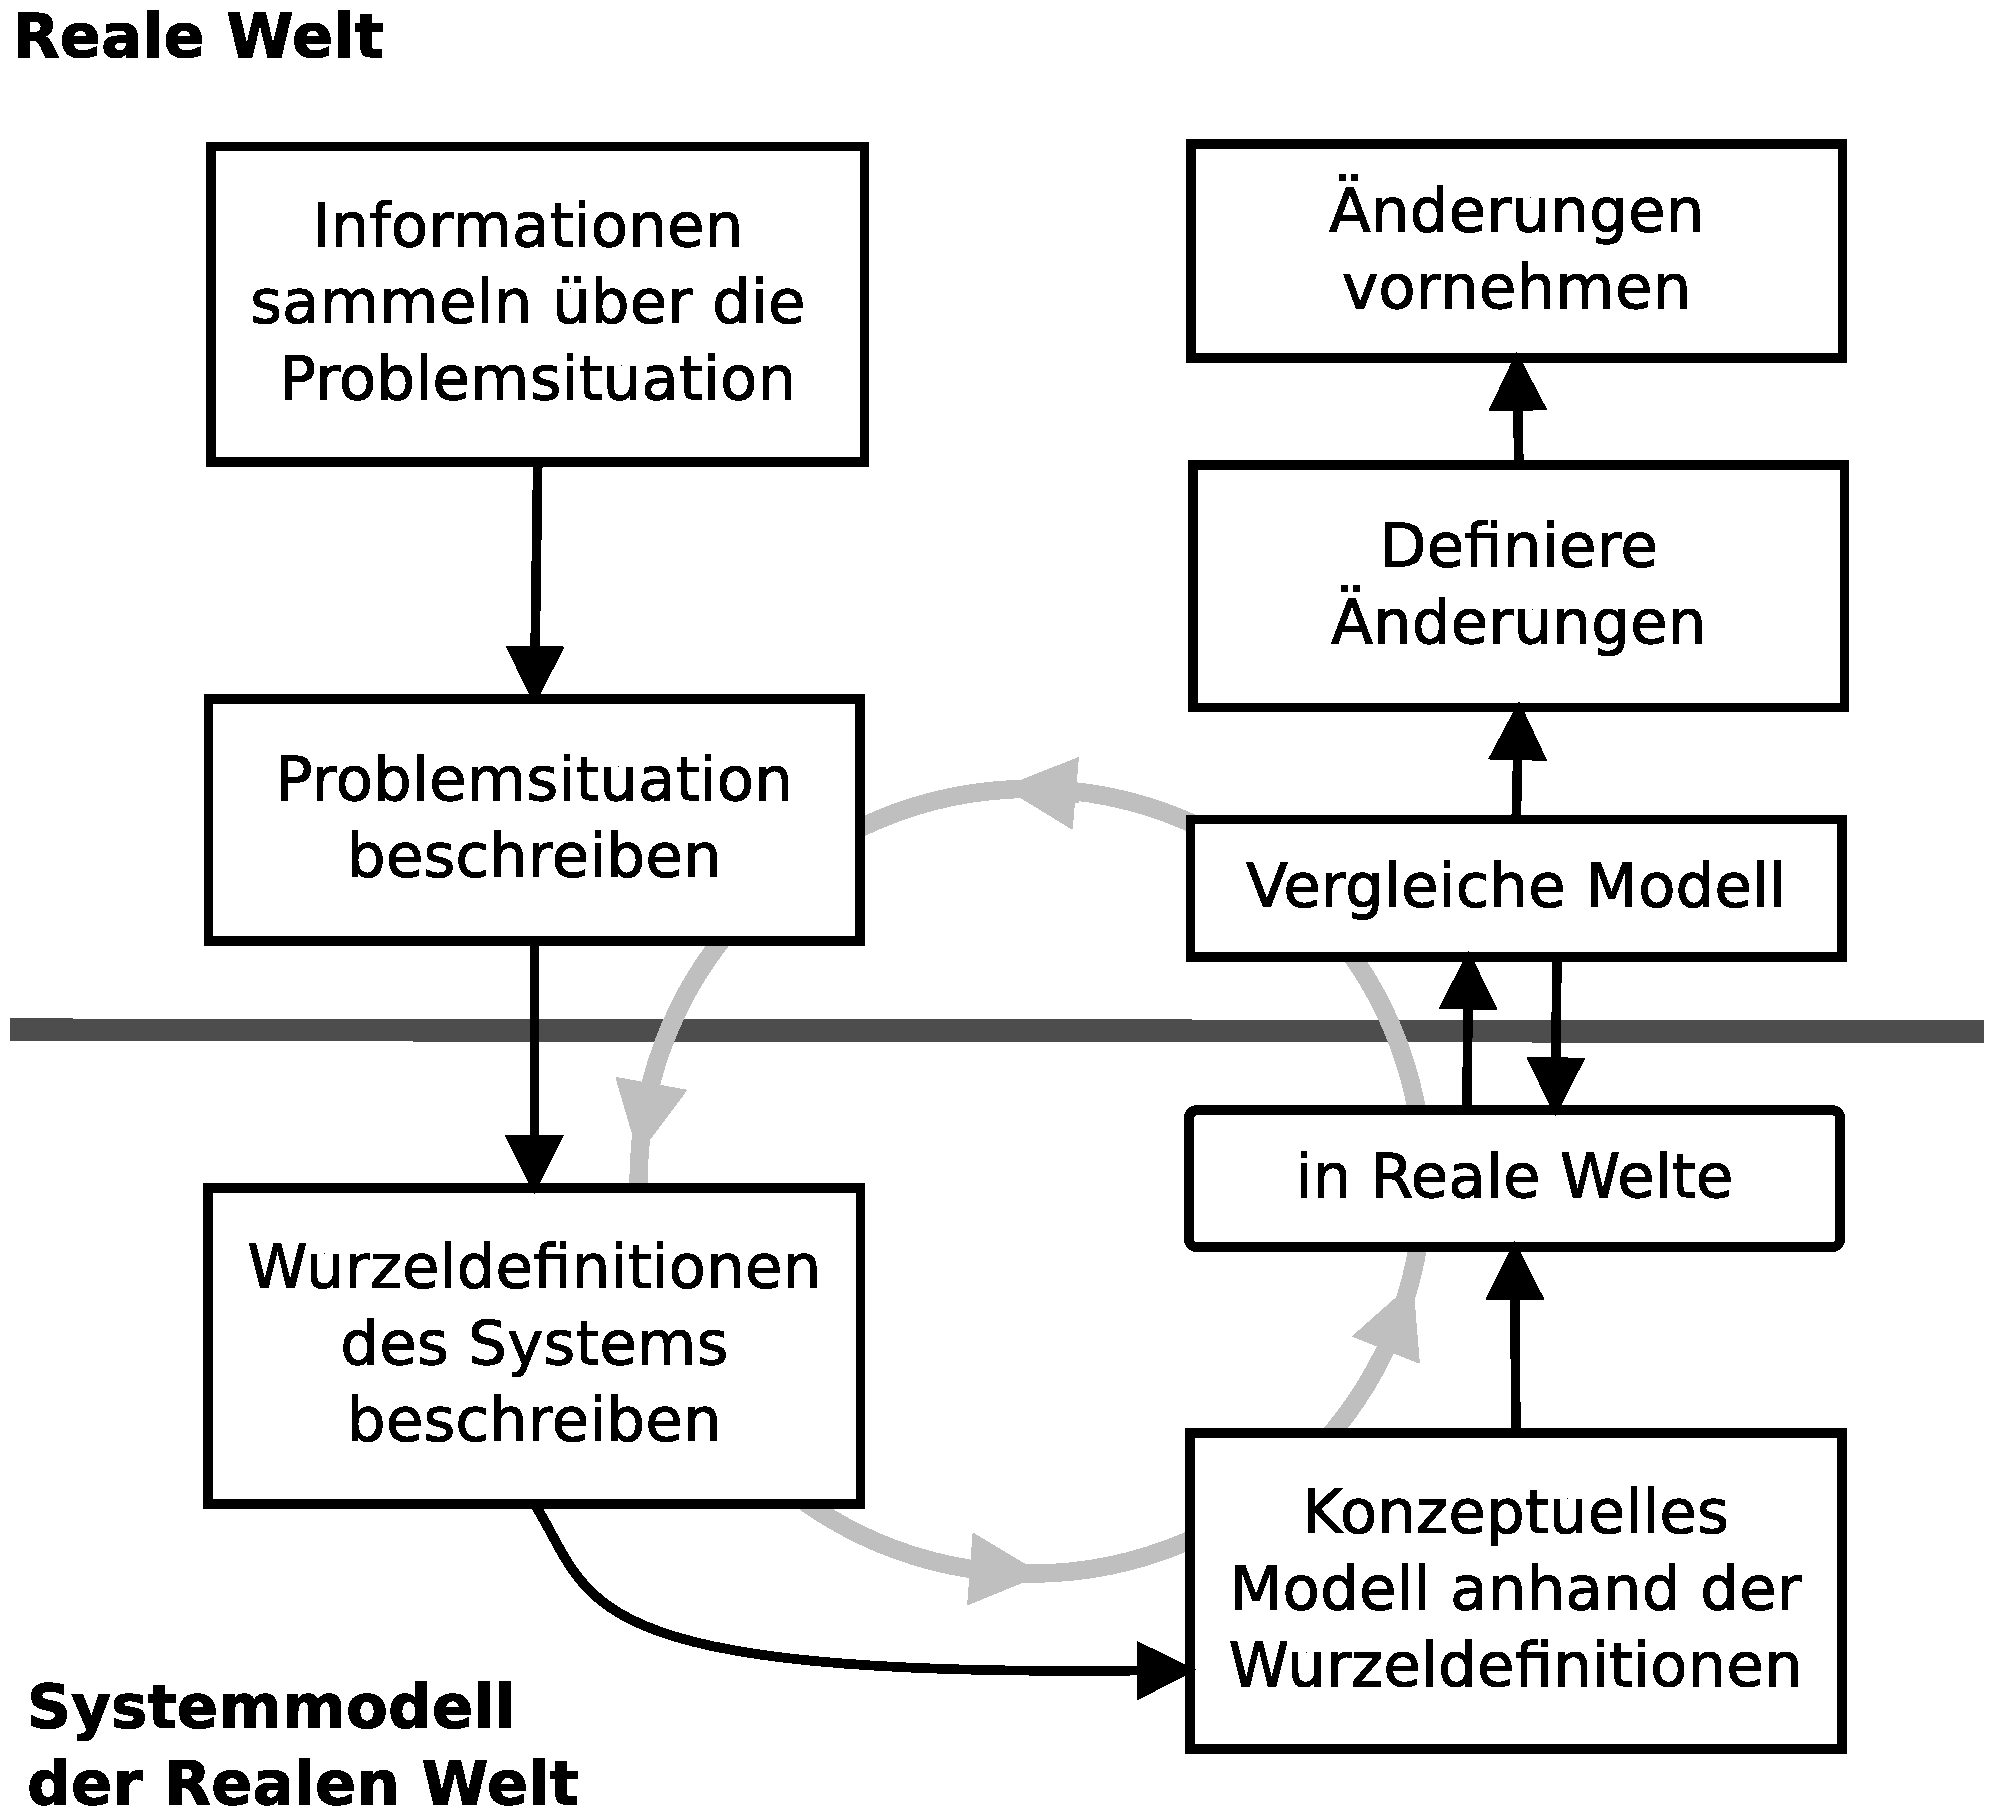
\includegraphics[scale=0.9]{images/ssm.pdf}
\caption{Soft Systems Methodologie}
\label{fig:ssm}
\end{figure}

Die Folgenden Inhalte sind den Quellen \cite{checkland, bobwill, ssmger} entnommen. Die Entwicklung von SSM begann in den späten 60iger Jahren an Universität von Lancaster und wurde von Peter Checkland geleitet. Es war zunächst als Modellierungswerkzeug gedacht, wird aber hauptsächlich als Lern- und Bedeutungswerkzeug angesehen, denn SSM kann prinzipiell immer dann eingesetzt werden, wenn jemand versucht, zielgerichtet zu handeln. Das Forscherteam um Peter Checkland hat SSM, beispielsweise während des Flugzeug-Projekt Concorde eingesetzt, bei welchem Sie beauftragt wurden zu helfen. Ein wichtiger Teil von SSM ist die Weltansicht, welche einem Vorgehen Sinn und Zweck verleiht. Beispielsweise ist des einen Terrorist des anderen Freiheitskämpfer. Beide Weltansichten betrachten jedoch dasselbe Geschehen. Durch mehrere zielgerichtete Vorgehen, unterschiedlicher Weltansichten, wird in SSM versucht, die Reale Welt zu beschreiben. Diese ist jedoch viel zu komplex, um in irgendeiner Modellsprache erfasst zu werden. Daher wird das Vorgehen bewusst auf ein rein konzeptionelles Modell beschränkt. Diese Einschränkung verringert die Komplexität und vereinfacht dadurch die Problemlösung. Die Abbildung~\ref{fig:ssm} zeigt die Schritte des SSM-Modells in drei Phasen. Die Trennung zwischen Realer Welt und Systemmodell der Realen Welt findet zwischen Phasen eins und zwei statt. In der ersten Phase wird die gesamte Problemsituation der Realen Welt aus Sicht aller Beteiligten erörtert und unstrukturiert beschrieben. Anhand dieser Informationen wird in der zweiten Phase ein Bild, in SSM-Terminologie Rich-Picture, erstellt. Dieses ist ein wichtiges Hilfsmittel zur Beschreibung der Problemsituation, welches möglichst viele Informationen in einem Bild erfassen soll. Mit dessen Hilfe sollen Grenzen, Struktur, Informationsflüsse, Kommunikationskanäle und das menschliche Aktivitätssystem eines Systems aufzeigt werden. Das Bild dient als Grundlage für die Ursachendefinitionen, welche einen festen Rahmen für die konzeptionellen Modelle ermöglichen. Die Ursachendefinitionen sorgen dafür, dass wichtige Aspekte nicht weggelassen werden. Die Gedächtnisstütze CATWOE\footnote{Übersetzungen wurden aus dem Artikel \cite{ssmger} übernommen.} ist eine Empfehlung zur Erstellung der Ursachendefinitionen:

\begin{itemize}[leftmargin=*]
\item \textbf{Client (Kunde)}, Wer oder Was profitiert von dem Umwandlungsprozess.
\item \textbf{Actor (Akteur)}, Wer ermöglicht den Kunden den Umwandlungsprozess.
\item \textbf{Transformation process (Umwandlungsprozess)}, von einem Startzustand in eine Endzustand.
\item \textbf{Weltanschauung}, gibt dem Umwandlungsprozess Bedeutung.
\item \textbf{Owner (Inhaber)}, vor Wem muss sich das System verantworten und/oder Wer kann veranlassen, dass es nicht existiert.
\item \textbf{Environmental constraints (Umweltauflagen)}, Was beeinflusst das System, ohne es zu kontrollieren.
\end{itemize}

Die Rollen welche Kunde, Akteur und Inhaber belegen, können in bestimmten Fällen überlappen. CATWOE ist keine willkürlich Ansammlung von Eigenschaften, sondern resultiert aus Beobachtungen der Realen Welt. Bei der Ausübung von SSM ist aufgefallen, dass insbesondere Akteur und Inhaber bei der Betrachtung ausgelassen werden, da diese "zu offensichtlich" erscheinen \cite[s.~255]{gutmann}. Die Reihenfolge, in welcher die Eigenschaften abgearbeitet werden, ist beliebig. Je nach Problemsituation sind einige Eigenschaften offensichtlicher als andere. Die konzeptuellen Modelle, welche aus den Ursachendefinitionen gebildet wurden, dienen dazu, Debatten über die Thematik zu strukturieren, indem sie mit der Realen Welt verglichen werden. In einem iterativen Prozess werden die ersten beiden Phasen wiederholt, bis die Thematik klar genug ist, um Ergebnisse zu treffen. Die Ergebnisse werden abschließend, in Phase drei, in konkrete Schritte formuliert, die ausgeführt werden sollen.

Die Soft Systems Methodology ist zwar keine Methodik, die explizit zur Erstellung eines Sicherheitskonzeptes gedacht ist, ihre Vorgehensweise für die Analyse, durch Trennung von Realer Welt und deren Abstraktion ist jedoch gut geeignet zum Lösen von Problemstellungen. SSM nimmt bewusst Einfluss auf das menschliche Denken und Vorgehen, um dieses zu fokussieren und dadurch zu optimieren.

\subsubsection{Data Flow Diagramme}

Der nachfolgender Paragraph bezieht sich auf \cite[s.~263]{gutmann}.
Durch die Bedrohungsanalyse (Kapitel~\ref{chap:threat_analysis}) mittels SSM wird geklärt, gegen welche Bedrohungen geschützt werden soll und welche Maßnahmen dafür notwendig sind. Darauf aufbauend kann die Bedrohungsmodellierung der Implementierung, unter Verwendung von Data Flow Diagrammen, angewandt werden. Data Flow Diagramme (DFD) gehen zurück auf die 70er Jahre. Ihre Aufgabe ist es, die gefährdeten Informationen der Applikation zu identifiziert, die Bedrohungen zu finden und Maßnahmen dagegen zu treffen. Es gibt mehrere Level von DFDs, welche den Detailgrad des Diagramms bestimmen. Für die Bedrohungsmodellierung reicht Level 0 aus. Es zeigt den Informationsfluss zwischen internen und externen Anwendungsgrenzen. Für die Bedrohungsmodellierung wird der Aufbau der Diagramme auf die fünf Objekte in Abbildung~\ref{fig:dfd_intro} beschränkt. Die Vertrauensgrenze ist ein Objekt, dass die klassische DFDs erweitert, um den Aspekt der Bedrohungen eines System darstellen zu können. Generell gilt, überschreitet eine Datenfluss eine Vertrauensgrenze, ist er durch Bedrohungen verwundbar.

\begin{figure}[htbp]
\centering
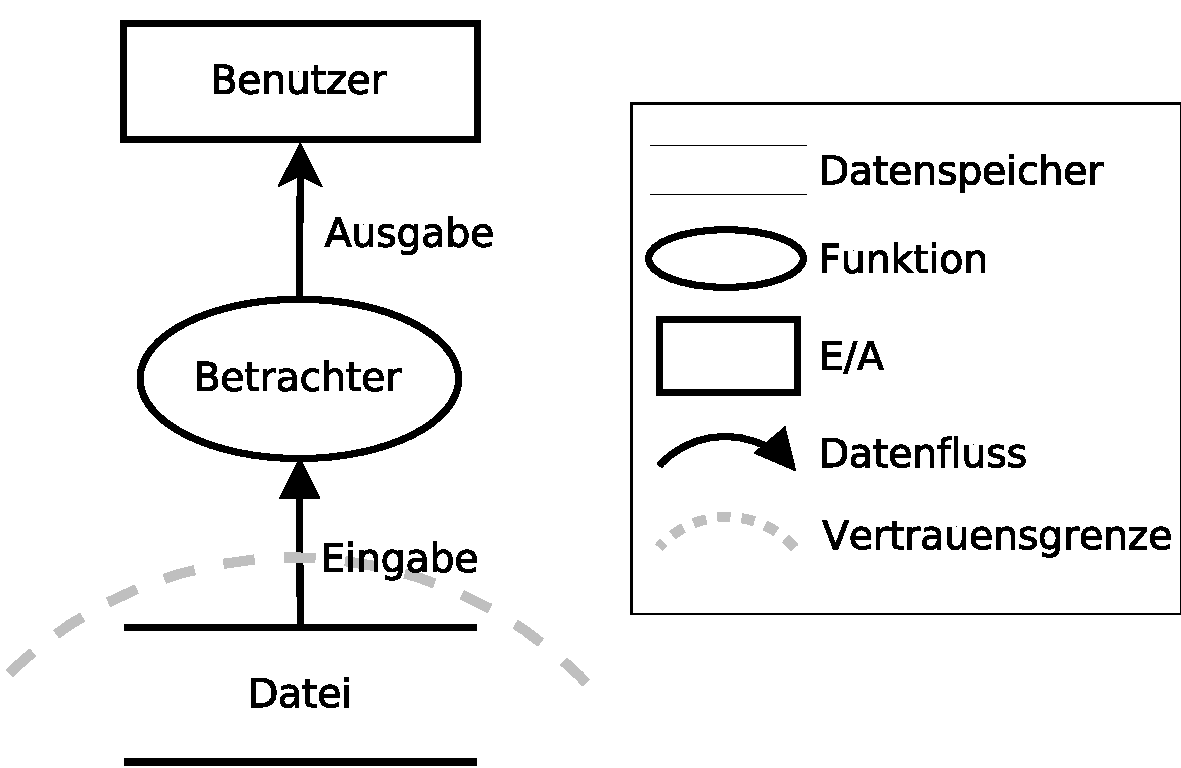
\includegraphics[scale=0.4]{images/dfd_intro.pdf}
\caption{Data Flow Diagramm Beispiel}
\label{fig:dfd_intro}
\end{figure}

Anhand der Data Flow Diagramme werden Gefährdungen für Informationsflüsse gesucht. Diese werden zunächst einfachheitshalber in fünf Kategorien gegliedert werden:

\begin{table}[h] % htbp ~ here, top, bottom, page
\begin{tabularx}{\linewidth}{@{}lX@{}}
\textbf{Sabotage} & unentdeckt Daten modifizieren\\
\textbf{Personifikation} & vorgeben, jemand oder etwas Anderes zu sein\\
\textbf{Informationspreisgabe} & unberechtigter Zugriff auf Informationen\\
\textbf{Disput} & meiden der Verantwortung für ein Tun oder Nichttun\\
\textbf{Denial of Service} & einen Service an seiner Ausübung hindern\\
\end{tabularx}
\end{table}

Denial of Service (DoS) ist eine zu allgemeine Gefährdung, sodass ausgehend von den Anderen vier, je nach Anwendungsfall, eine detailliertere Analyse statt findet.

\section{Authentifizierungsverfahren} \label{sec:auth_modells}

Für die Authentifizierung gibt es verschiedene Möglichkeiten, diese unterscheiden sich sowohl in ihrem Aufwand als auch ihrem Nutzen.

\paragraph{Vertrauen}

Vertrauen ist der Zustand, der durch Authentifizierung erreicht werden soll. Vertrauen sagt aus, das ein Partner einem anderen Partner in Funktion, Ehrlichkeit und Zuverlässigkeit, aufgrund von eigenen Erfahrungen, glaubt \cite{chen}. Dabei unterscheidet man einseitiges und beidseitiges Vertrauen. Von einseitigem Vertrauen wird gesprochen, wenn nur ein Partner einen Nachweis seiner Identität erbracht hat. Bei beidseitigem Vertrauen haben beide Kommunikationspartner gegenseitig überprüft, dass der Andere derjenige ist welcher er vorgibt zu sein.

\paragraph{Passwörter}

Bei passwortbasierter Authentifizierung weist sich ein Kommunikationspartner über einen eindeutigen Namen und ein Passwort gegenüber einem anderen Kommunikationspartner aus. Passwortbasierende-Authentifizierung wird meistens Verwendet, um einseitig Vertrauen herzustellen. Der typische Einsatz ist die Anmeldung an einem Server, um zugriff auf dessen Services zu erhalten. Der Benutzer weißt sich mit Name und Passwort gegenüber dem Server aus, umgekehrt gibt es oft keinen Nachweise über die Identität. Eine Möglichkeit des Identitätsnachweises von Serverseite sind Zertifikate (vgl.~\ref{sec:auth_asym}). Die Sicherheit von Passwörtern basiert auf der Annahme, dass der Benutzer ein sicheres Passwort gewählt hat und dieses stets vor fremden Zugriff schützt. Die Realität zeigt jedoch, dass diese Annahme selten zutrifft \cite[s.~2]{gutmann}.

\paragraph{Symmetrisch}

Symmetrische Verfahren arbeiten mit einem Passwort oder Schlüssel, der beiden Kommunikationspartnern bekannt ist. Dieser muss vor der Kommunikation, über einen zweiten Kanal, etwa persönlich, ausgetauscht werden. Das Verfahren wird deshalb auch als Pre-Shared-Key (PSK) bezeichnet. Die verbreitete Anwendung von PSKs sind WLAN-Netzwerk im Privaten Bereich. Zugang zu einem solchen WLAN-Netzwerk kann jeder erhalten, der den Schlüssel kennt. Unter der Annahme, dass nur Berechtigte den Schlüssel kennen wird ein Vertrauensverhältnis zwischen den Kommunikationspartnern in dem Netzwerk aufgebaut. Bei steigender Anzahl der Kommunikationspartner wird dieses System unbrauchbar, denn jeder neue Partner erhält den gleichen Schlüssel. Soll nun einem Berechtigten der Zugriff verboten werden muss der Schlüssel gewechselt werden. Dies führt dazu das alle, außer derjenige dem die Berechtigung entzogen wurde, diesen neuen Schlüssel benötigen.

\paragraph{Asymmetrisch} \label{sec:auth_asym}

Asymmetrische Verfahren arbeiten mit zwei Schlüsseln, einem Öffentlichen und einem Privaten. Damit generierte Schlüssel möglichst einzigartig sind, wird eine Zufallszahl verwendet (Abbildung~\ref{fig:pp_keygen}). Der Öffentliche Schlüssel wird dem Kommunikationspartner übergebenen. Der Private Schlüssel bleibt im eigenen Besitz und wird vor fremden Zugriff geschützt. 

\begin{figure}[htbp]
\centering
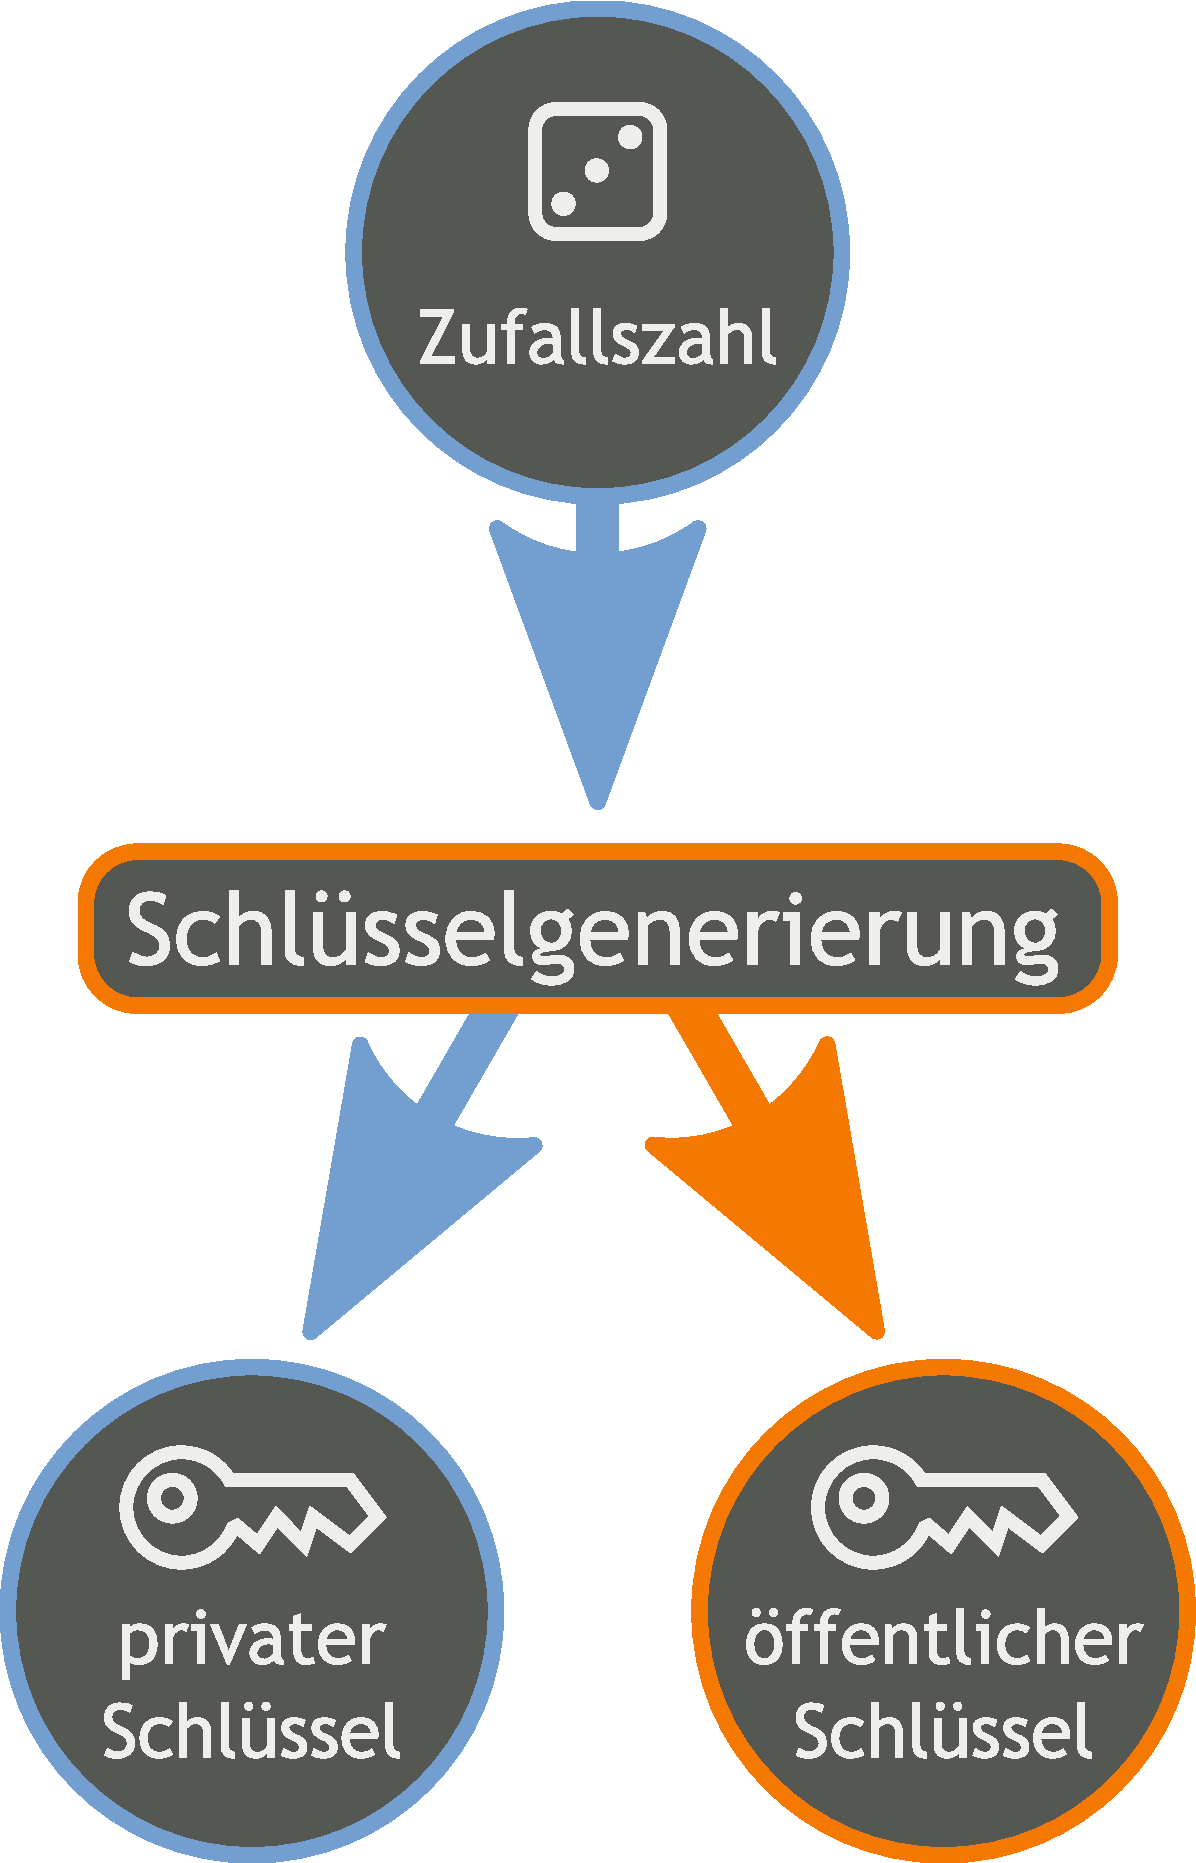
\includegraphics[scale=0.2]{images/public_private_keygeneration.pdf}
\caption{Public/Private Schlüsselgenerierung aus \cite{wiki_asym_crypto}}
\label{fig:pp_keygen}
\end{figure}

Der große Vorteil dieses Verfahrens gegenüber den Symmetrischen ist, das der Öffentliche Schlüssel über einen nicht vertrauenswürdigen Kanal geteilt werden kann. Bei der Authentifizierung wird der private Schlüssel genutzt, um eine Nachricht zu signieren. Mit dem Öffentlichen Schlüssel kann der Kommunikationspartner verifizieren, dass die Nachricht von dem Kommunikationspartner kommt, der den passenden privaten Schlüssel hat (Abbildung~\ref{fig:pp_veri}). Dadurch kann festgestellt werden, ob die Nachricht auf dem Transportweg manipuliert worden ist, allerdings bleibt das Problem des Vertrauens, denn ob der Schlüssel von demjenigen stammt, der der Kommunikationspartner vorgibt zu sein, ist dadurch nicht garantiert. Hierbei wurde die Notwendigkeit nach einem expliziten Austauschkanal eliminiert, da der Schlüsselaustausch, über einen unsicheren Kanal erfolgen kann. Allerdings hat man dadurch das Bedürfnis nach einen Authentifizierungskanal geschaffen, um eine Identitätsprüfung durchführen zu können.
 
\begin{figure}[htbp]
\centering
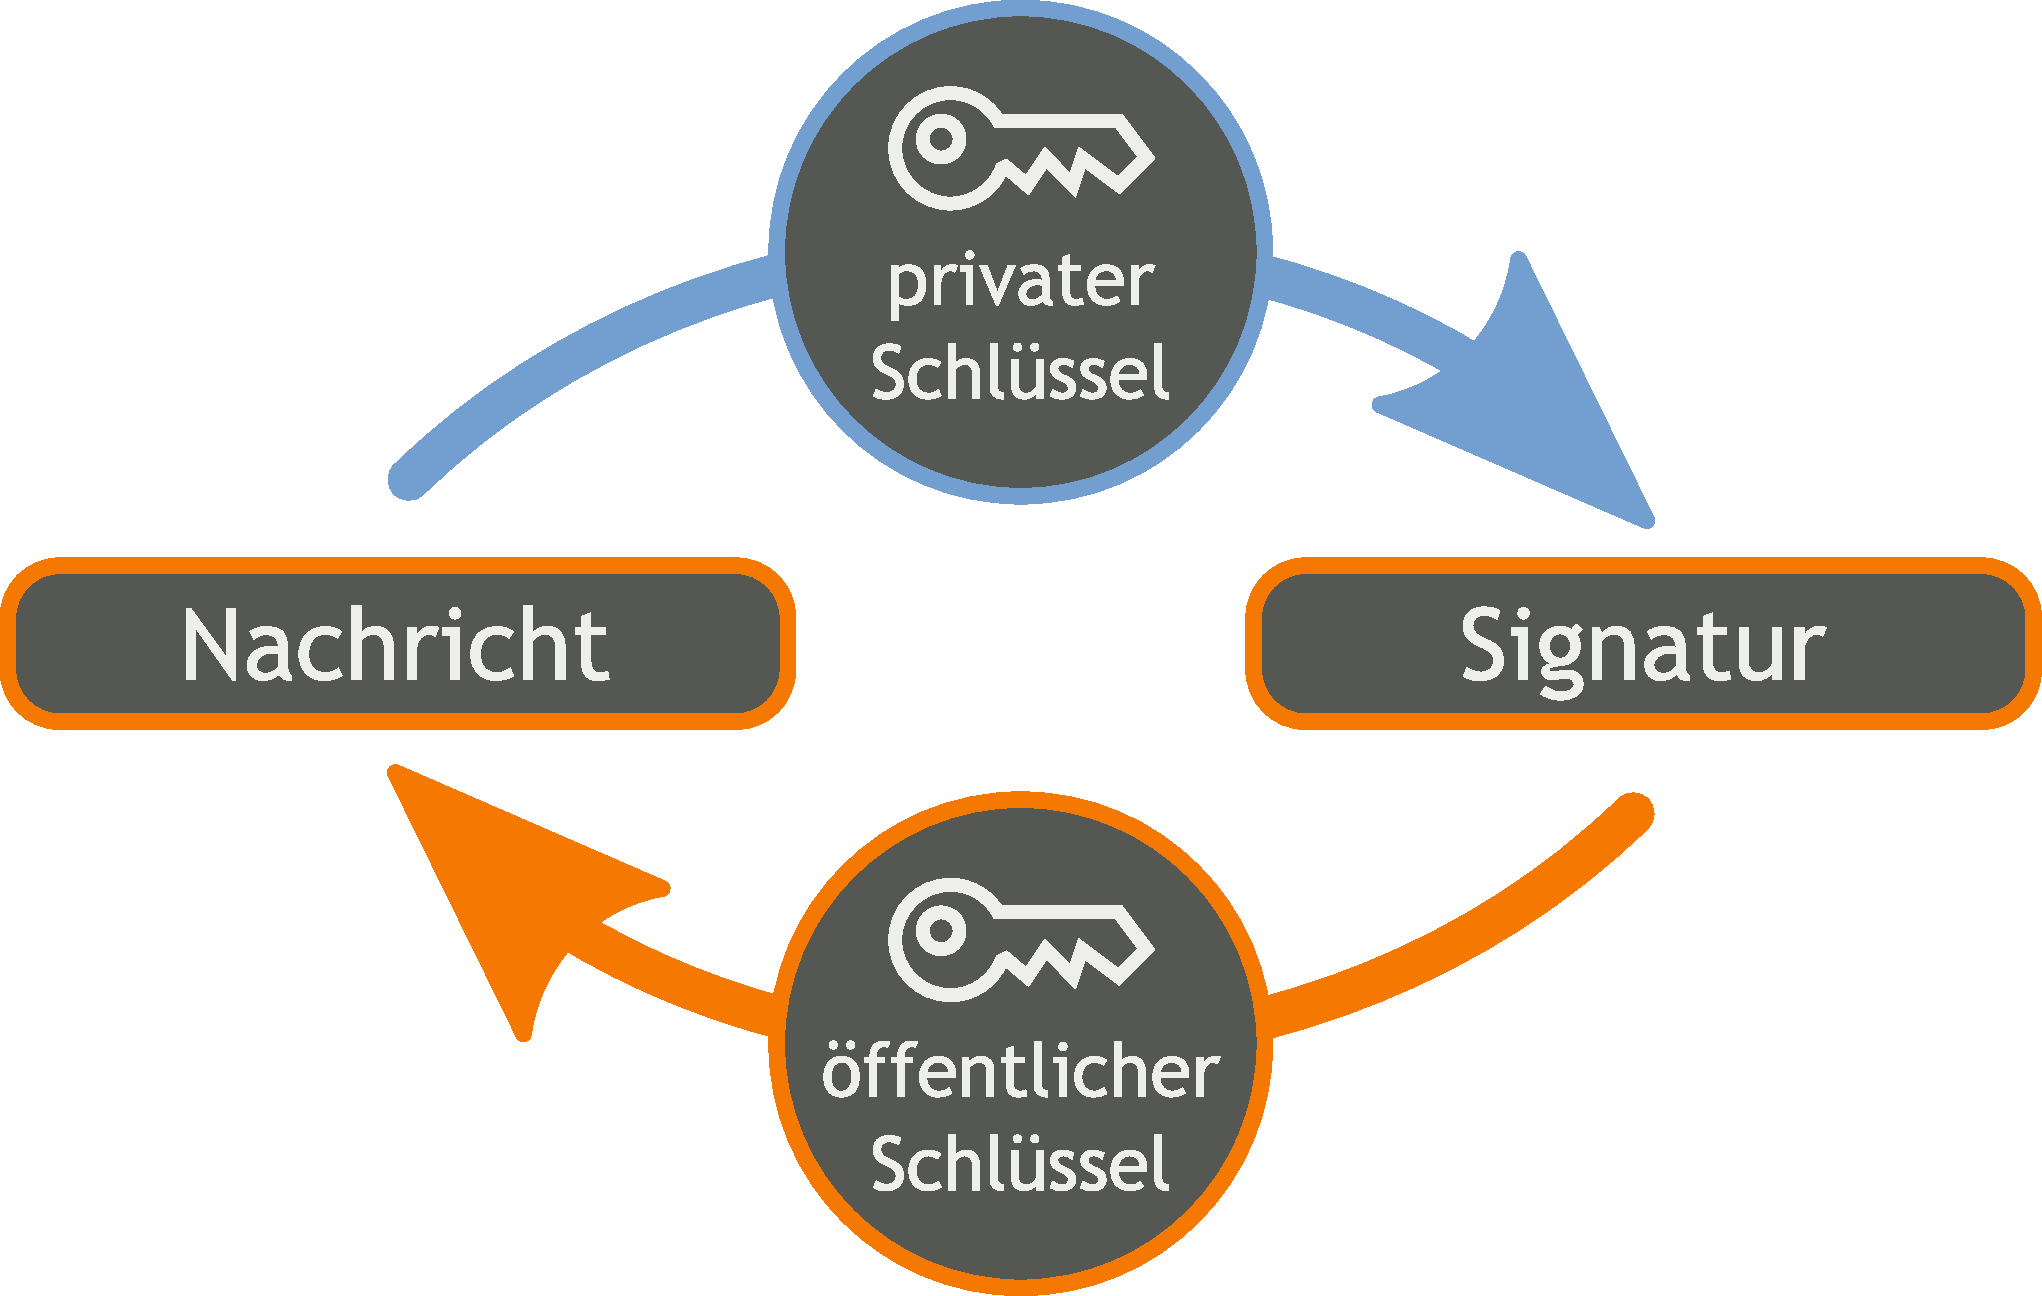
\includegraphics[scale=0.2]{images/public_private_verification.pdf}
\caption{Public/Private Verifizierung aus \cite{wiki_asym_crypto}}
\label{fig:pp_veri}
\end{figure}

Aus diesem Hintergrund wurden Zertifikate erschaffen, der heutige verbreitetste Standard sind Zertifikate im X.509-Format. Ein Zertifikat beinhaltet Informationen über den Inhaber, die Zertifizierungsstelle, die Gültigkeit und den Öffentlichen Schlüssel. Anstatt den Öffentlichen Schlüssel auszutauschen, wird nun das Zertifikat gesendet. Bei der Zertifizierungsstelle kann die Echtheit sichergestellt werden. 

\chapter{Vorgehensweise}

\section{Zielsetzung}

Ziel dieser Thesis ist es, eine Lösung zur Authentifizierung und Autorisierung für den Fernzugriff auf den Marktrechner zu schaffen. Abbildung~\ref{fig:uc_solution} zeigt die relevanten Use-Cases. Auf der linken Seite sind die Benutzer zu sehen, diese wollen lokal oder remote bestimmte Funktionen auf dem Marktrechner aufrufen. Dazu müssen Sie vorher authentifiziert und autorisiert werden. Die Autorisierung soll auf einem Rollenmodell basieren, wobei ein Benutzer mehrere Rollen inne haben kann. Die Benutzung über den Reumotezugriff soll über HTTPS und das RestGateway des Marktrechners erfolgen. Zur Überprüfung der Authentifizierungs- und Autorisierungsdaten des Nutzers soll ein Authentifizierungs- und  Autorisierungs-Server (AAS) kontaktiert werden. Dieser AAS kann räumlich getrennt von den Benutzern, etwa über das Internet erreichbar sein. Der Marktrechner soll die Möglichkeit bieten mehrere AAS Anfragen zu können.

\begin{figure}[htbp]
\centering
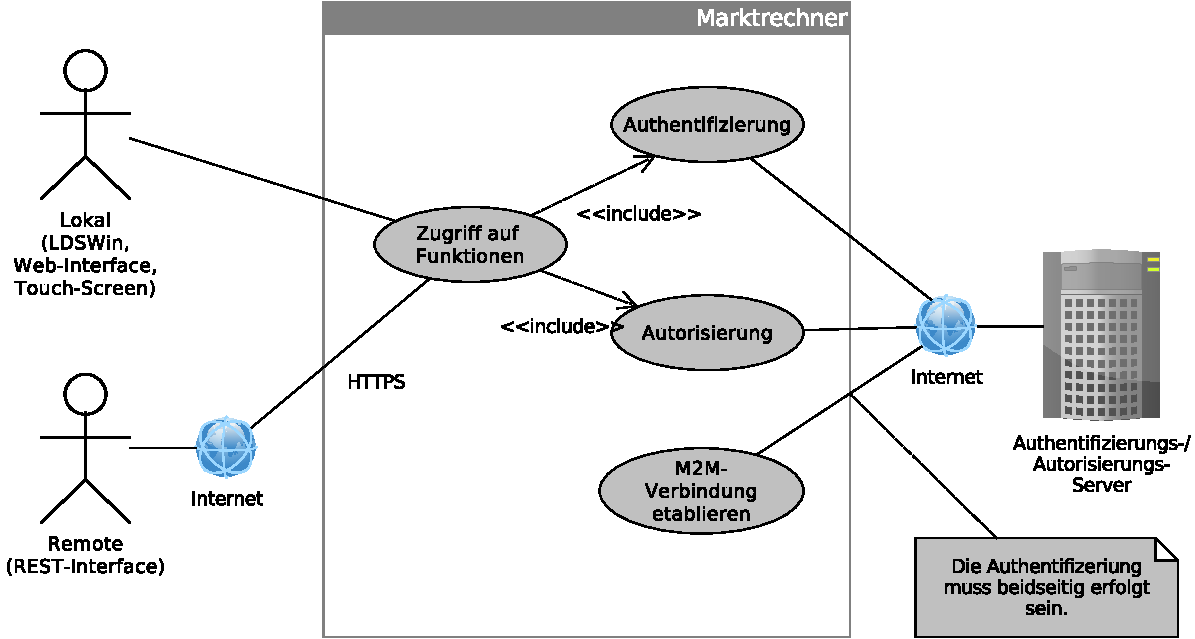
\includegraphics[scale=0.6]{images/ziel_usecase.pdf}
\caption{Zielsetzung Use-Case-Diagramm}
\label{fig:uc_solution}
\end{figure}

\section{Schritte}

Im Grundlagenteil~\ref{sec:sec_standard} wurde mit den Common Criteria ein Sicherheitsstandard vorgestellt, welcher für die Entwicklung sicherer Systeme angewendet wird. Das für diese Thesis relevante Protection Profile analysiert, die aus Kundensicht relevanten Anforderungen des zu sichernden Systems. Ein komplettes PP zu erstellen würde den Rahmen der Thesis sprengen, deswegen werden die wichtigsten Aspekte herausgenommen und behandelt. Dazu werden zunächst die zu schützenden Güter und deren Bedrohungen analysiert. Anschließend werden Lösungsvorschläge zu den Bedrohungen getätigt. Dabei soll unbedingt vermieden werden, Bezug auf eine bestimmte Technologie zu nehmen, außer es gibt nur eine zulässige Lösung. Zum Schluss werden noch Kriterien aufgestellt anhand welcher die Evaluierung durchgeführt werden soll.

\section{Methoden}

Als Methoden für die Bedrohungsanaylse werden die Soft Systems Methodology und Data Flow Diagramme eingesetzt. Unterstützend werden Gefährdungenkataloge und Maßnahmenkataloge aus dem IT-Grundschutz des BSI herangezogen. Dessen Vorarbeit, in welchen IT-Systemen, welche Bedrohungen auftreten können und die Maßnahmen dazu, sind eine gute Quelle, die eine größere Abdeckung von Bedrohungen in dieser Thesis ermöglichen.

\chapter{Bedrohunganalyse} \label{chap:threat_analysis}
\epigraphhead[70]{\epigraph{The only truly secure system is one that is powered off, cast in a block of concrete and sealed in a lead-lined room with armed guards.}{\textit{Gene Spafford}}}

Die Bedrohungsanalyse gliedert sich in die drei SSM-Phasen, die in Abschnitt~\ref{sec:ssm} beschrieben sind. Zunächst wird die Problemsituation beschrieben, danach werden zwei konzeptionelle Modelle aus unterschiedlichen Weltansichten erstellt. Die unterschiedlichen Weltansichten entstammen der Betrachtung eines Beschützers und eines Angreifers des Systems. Durch den Vergleich der konzeptionellen Modelle mit der Realen Welt werden konkrete Maßnahmen formuliert. Das Ergebnis der Bedrohungsanalyse soll mögliche Bedrohungen aufdecken und erste Maßnahmen formulieren.

\section{Beschreibung der Problemsituation} \label{sec:problem_situation}

Die in Abschnitt~\ref{sec:marktrechner} geschilderte Architektur des Marktrechnerumfeldes, wird mit dem Rich-Picture in Abbildung~\ref{fig:problem_situation} auf Sicherheitsmängel untersucht. Der Fokus dieser Arbeit liegt auf dem Fernzugriff, dennoch werden auch die Probleme des lokalen Zugriffes erfasst. Dadurch soll verhindert werden, dass der Fernzugriff unnötige Hindernisse für die lokale Zugriffskontrolle schafft. 

\begin{figure}[htb]
\centering
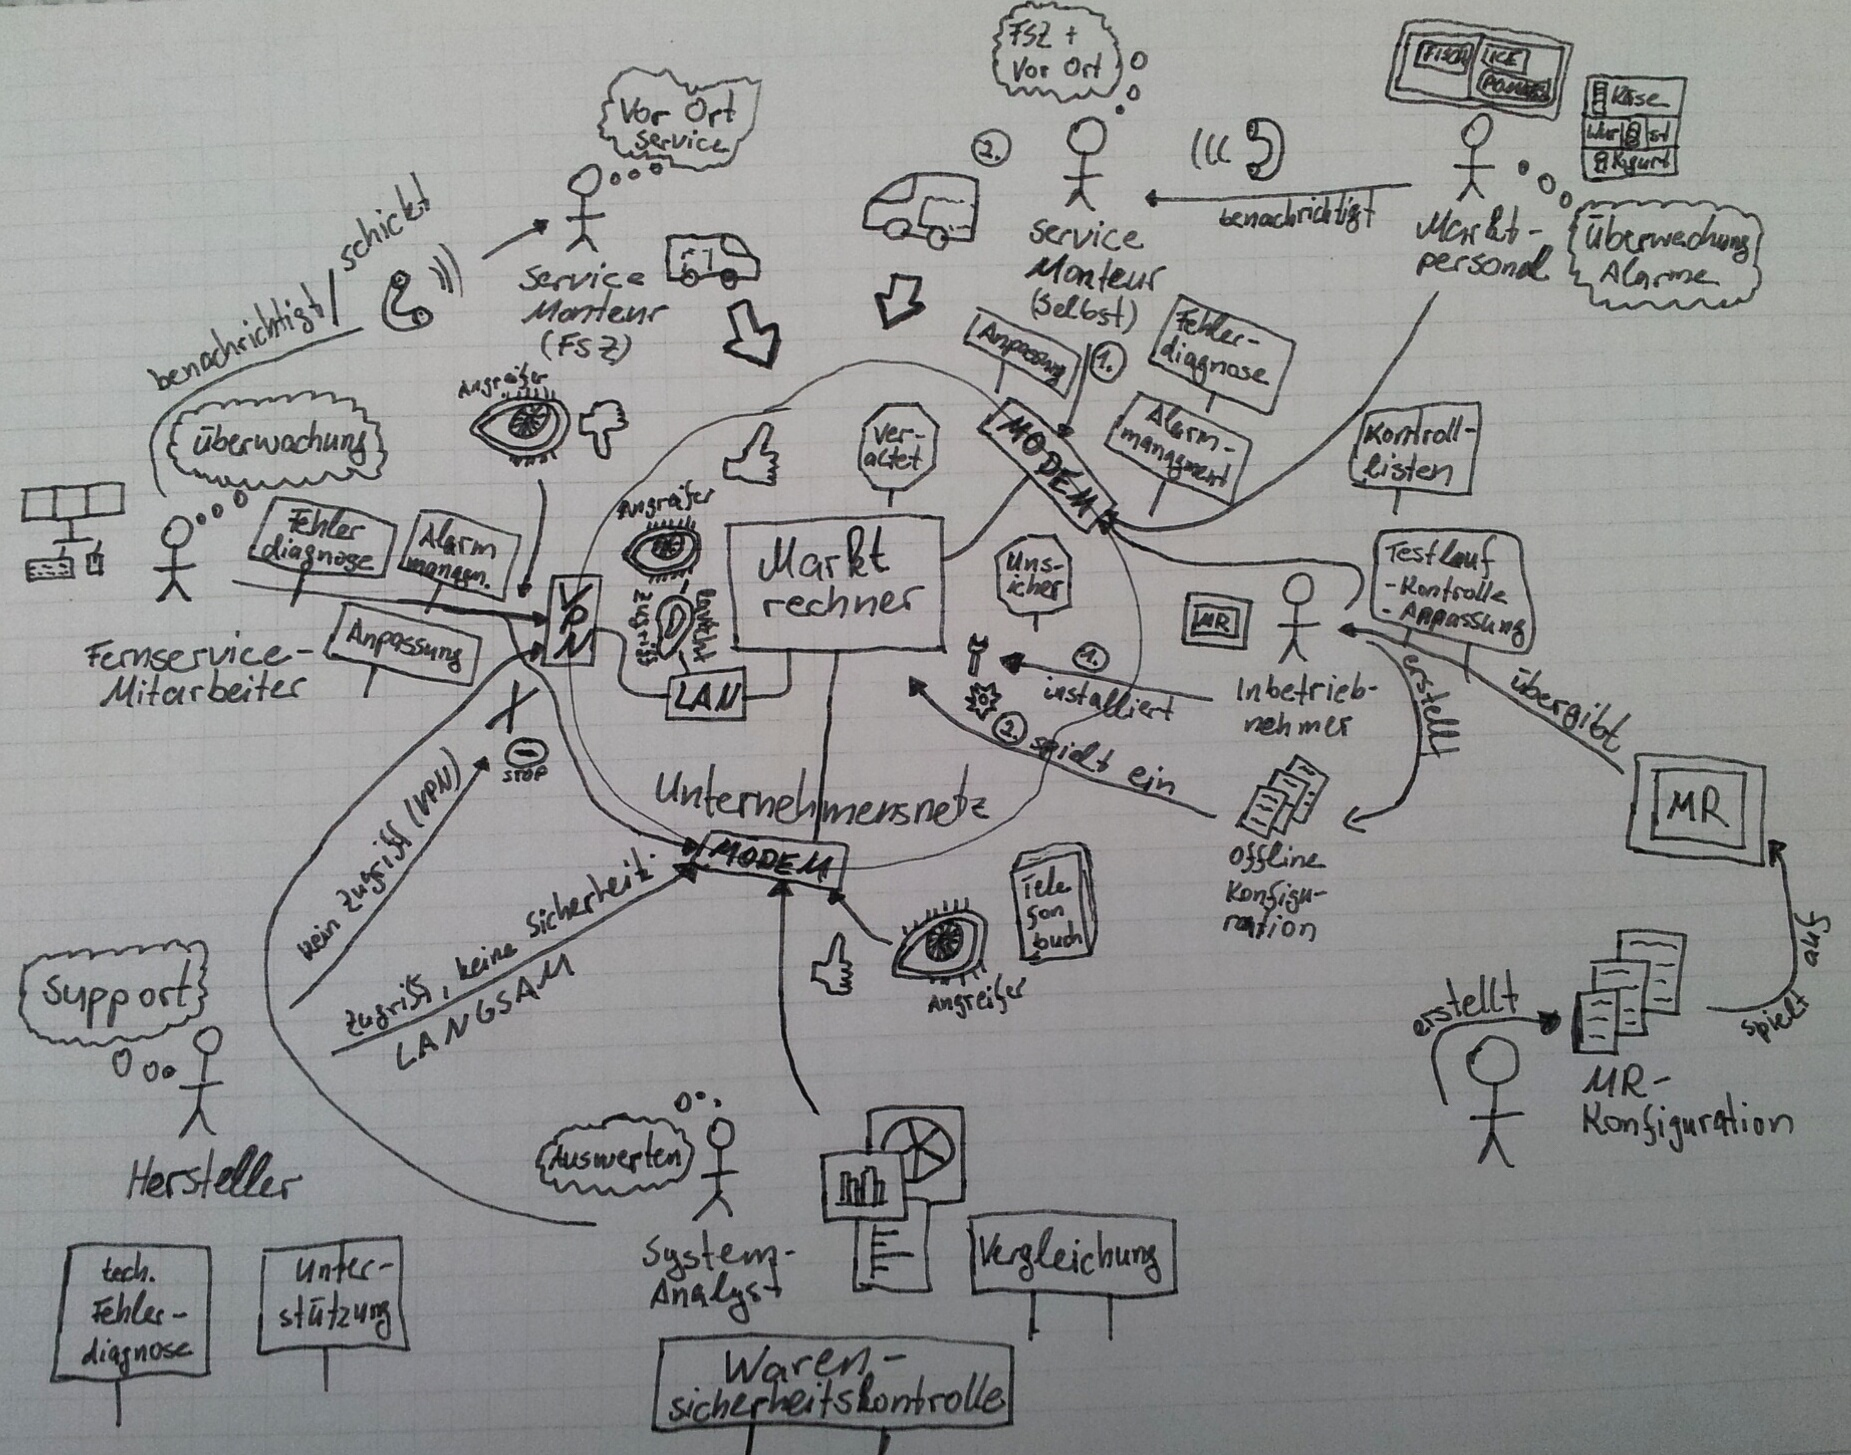
\includegraphics[scale=0.215]{images/problemsituation.jpg}
\caption{Problemsituation}
\label{fig:problem_situation}
\end{figure}

\subsection{Identifizieren der Rollen} \label{sec:roles}

Zunächst wird ein Überblick über alle Zugriffsberechtigten geschaffen. Diese werden anhand von Rollen zusammengefasst, welche Funktion und Zugriffsart beschreiben. Alle Rollen sind in der Abbildung~\ref{fig:problem_situation} illustriert. Die Beschreibungen der Rollen sind allgemein gehalten und nehmen keinen Bezug auf aktuelle oder zukünftige technologische Begebenheiten.

\paragraph{Der Projektierer} konzipiert und entwirft komplette Kälteanlagen. Ein Teil seiner Aufgabe kann das Erstellen der Offline-Konfiguration sein. Diese kann direkt von Werk aus aufgespielt werden. Der Inbetriebnehmer muss den vorkonfigurieren Marktrechner dann lediglich noch installieren und testen.

\paragraph{Der Inbetriebnehmer} ist die Rolle, welche das System initial zum Laufen bringt. Der Inbetriebnehmer muss vor Ort die Anlage in Betrieb nehmen. Dazu kann er bereits im Voraus eine Offline-Konfiguration anlegen, welche an die Anlage des Kunden angepasst ist. Die Konfiguration wird auf die Anlage eingespielt, sobald die Hardware installiert ist. Bevor die Anlage produktiv eingesetzt werden kann, wird ein Testlauf durchgeführt. Während des Testlaufs muss der Inbetriebnehmer die Anlage überwachen, um bei Problemen die Konfiguration, die Parameter und die Einstellungen anzupassen. Zur Überwachung des Testlaufes muss der Inbetriebnehmer nicht zwingend permanent vor Ort sein, sondern kann den Status auch aus der Ferne abrufen, damit der Inbetriebnehmer nicht etliche Stunden neben dem Marktrechner auf das Auftreten von Fehlern warten muss.

\paragraph{Der Service-Monteur} führt Wartungen und Störungsbehebungen durch. Für den Service-Monteur gibt es zwei denkbare Ausprägungen. Als Selbständiger wird er im Fall einer Störung durch den Eigentümer der Anlage oder dessen Personal benachrichtigt. Nun hat er die Möglichkeit, aus der Ferne eine Fehlerdiagnose durchzuführen und Veränderungen an der Konfiguration und dem Alarmmanagement durchzuführen. Sollte er nicht in der Lage sein, die Störung aus der Ferne zu beheben, muss er die selbe Tätigkeiten vor Ort durchführen können. Als Mitarbeiter im Außendienst einer Fernservice-Zentrale entfällt die Diagnose und die Fehlerbehebung aus der Ferne, da dies bereits durch den Fernservice-Mitarbeiter durchgeführt wurde. Wenn die Störung von dort nicht gelöst werden kann, wird der Service-Monteur zur Anlage geschickt.

\paragraph{Der Fernservice-Mitarbeiter} überwacht mehrere Anlagen aus der Ferne. Diese Rolle führt die selben Tätigkeiten wie ein Service-Monteur durch. Allerdings erfolgt die bereits erwähnte Fehlerdiagnose, Kontrolle und Anpassung von Parametern und Einstellungen, sowie das Alarm-Management ausschließlich aus der Ferne. Einige Störungen können durch Anpassen der Konfiguration hinausgezögert werden, bis ein Service-Monteur vor Ort ist. Dadurch kann zum Beispiel Warenschaden auf Kosten von Energieeffizienz verhindern werden.

\paragraph{Der System-Analyst} wertet relevante und vergleichbare Daten zur Energieeffizienz und Warensicherheit aus. Auch er arbeitet ausschließlich aus der Ferne. Auswertbare Daten sind etwa Temperaturwerte oder Energieverbrauch. Sollten diese Werte im Vergleich mit anderen Anlagen negativ auffallen, kann er veranlassen, dass eine Anlage überprüft wird.

\paragraph{Der Eigentümer/Das Marktpersonal} ist daran interessiert, eine Kontrolle der Parameter zur Warensicherheit durchzuführen und eine Dokumentation der Waren-Temperaturen zu erhalten. Auch soll das Marktpersonal über Alarme informiert werden, um einen Service-Monteur zu benachrichtigen und Warenschaden zu verhindern. Die Rolle des Marktpersonals kann Zugriff vor Ort benötigen aber auch der Zugriff aus der Firmenzentrale wäre denkbar.

\paragraph{Der Hersteller} produziert die Hardware und entwickelt die Software des Marktrechner. Nach der Installation eines Marktrechner kann er anderen Rollen Unterstützung bei der Durchführung ihrer Arbeiten geben. Damit bei Softwareproblemen schnell Hilfe geleistet werden kann, will er sich aus der Ferne verbinden können	. 

\subsection{Systemumgebung}

Der Marktrechner wird als Teil einer Kälteanlage beim Kunden installiert und wird dort an dessen Netzwerk angeschlossen. Der Fernzugriff auf einen Marktrechner ist prinzipiell immer möglich. Zwei Arten des Fernzugriffs sind etabliert, über VPN oder Modem. Verbindungen über VPN kommen ausschließlich in Fernwarten zum Einsatz. Zum aktuellen Zeitpunkt sind etwa ein Viertel der Marktrechner über VPN erreichbar. Der Einsatz von VPN hat den Nachteil, dass er extrem aufwendig zu etablieren ist. Denn hier treffen unterschiedliche IT-Infrastrukturen zusammen, was ein Garant für Probleme ist. Beispielsweise sind Überschneidungen bei IPv4-Adressen eines der Hauptprobleme, da viele Administratoren Subnetze aus der Literatur übernehmen und diese diesbezüglich größtenteils gleich ist. Außerdem beschränkt sich der Zugriff ausschließlich auf die gekoppelten Netze. Dadurch ist es dem Hersteller nicht möglich, Unterstützung aus der Ferne zu leisten. Alle anderen Verbindungen werden über Modems ermöglicht. Deren Einsatz ist veraltet und bietet nur sehr geringe Übertragungsgeschwindigkeiten. Zudem stellen immer mehr Internet-Provider analoge ISDN-Anschlüsse auf Voice-over-IP (VoIP) Lösungen um. VoIP sorgt dafür, dass eine zuverlässige Modem-Kommunikation unmöglich wird. Über VPN ist die Verbindung bis zum Unternehmensnetz abgesichert, sodass ein Angreifer hier wenig Möglichkeit hat einzudringen. Die Modem-Verbindung stellt für einen Angreifer allerdings kaum ein Hindernis dar, da er lediglich die Telefonnummer kennen muss. Zusätzlich kann er die Modem-Leitung dauerhaft blockieren und dadurch unterbinden, dass andere Teilnehmer sich verbinden können. Durch oben genannte VoIP-Problematik, wird das Modem im Rahmen der Thesis nicht weiter berücksichtigt, da es absehbar abgelöst werden muss. Für das LAN, indem sich der Marktrechner befindet, gilt, dass ein Angreifer durch keine geeigneten Sicherheitsmaßnahmen aufgehalten wird.

\section{Sichtweise der Beschützer} 

Anhand der in Abschnitt~\ref{sec:problem_situation} beschriebenen Problemsituation wird hier die Sichtweise der Beschützer des Systems betrachtet. Zunächst legen die Ursachendefinitionen das Grundgerüst fest, in welchem sich die Beschützer bewegen. Anhand derer wird dann das Konzeptionelle Modell aufgebaut, das klare Anforderungen stellt, die die Beschützer für sinnvoll halten. Dieses Systemmodell wird abschließend mit der Realen Welt verglichen.

\subsection{Ursachendefinitionen}

Bei den Ursachendefinitionen der Beschützer sind die Eigenschaften für Kunden, Inhaber und Umwandlungsprozess offensichtlich. Für den Akteur, die Weltanschauung und die Umweltauflagen bedarf es hingegen einer genaueren Analyse:

\setlength{\tabcolsep}{12pt}
\renewcommand{\arraystretch}{1.5}
\begin{table}[h] % htbp ~ here, top, bottom, page
\begin{tabularx}{\linewidth}{@{}lX@{}}
\textbf{Kunden} & Alle Rollen aus Abschnitt~\ref{sec:roles} und der Marktrechner\\
\textbf{Inhaber} & Angreifer\\
\textbf{Umwandlungsprozess} & 
Von einem nicht vertrauenswürdigen Zustand in einen vertrauenswürdigen Zustand wechseln.\\
\end{tabularx}
\end{table}

\paragraph{Akteur} Diese Rolle kann je nach Dienstleister und Kundenwünschen unterschiedlich besetzt sein. Die offensichtlichsten Akteure sind Hersteller und Fernservice-Zentralen. Darüber hinaus wäre es denkbar, dass ein Marktbetreiber selbst diese Rolle einnehmen möchte.

\paragraph{Weltanschauung} Hersteller und Fernservice-Zentralen sind daran interessiert, unerwünschte Zugriffe zu verhindern und ihre jeweiligen vertraulichen Daten zu schützen. Das zu schützende Gut des Hersteller ist sein proprietäres Protokoll, da mit dessen Kenntnis unbemerkt Schaden angerichtet werden kann. Deshalb sollen die Kommunikationsinhalte geschützt werden, um zu verhinder das Angreifer Kenntnisse über Programmroutinen und Protokolle erlangen. Ein kompromittiertes Protokoll könnte ein Angreifer nutzen, um Warenschaden anrichten, wofür der Hersteller und/oder die Fernservice-Zentrale haftbar sein können. Darüber hinaus kann ein Imageschaden verursacht werden, um zum Beispiel Endkunden abzuwerben. Die Benutzer hingegen wollen ein funktionierendes System, sie haben einen Kältehintergrund und keine Ahnung von IT, Vertraulichkeit ist von sekundärer Natur. Wenn der Prozess, Vertrauen zu schaffen, Dinge kompliziert, wird der Benutzer versuchen ihn zu umgehen. Sollte das System nicht funktionieren, weil der Benutzer die Authentifizierung falsch bedient, ist trotzdem das System schuld, denn es ist seine Aufgabe, den Benutzer darauf hinzuweisen \cite[s.~5]{gutmann}. Zusätzlich spielt die Nachvollziehbarkeit eine große Rolle den durch das Wissen--"Wer hat wann mit welchen Mitteln was veranlasst beziehungsweise worauf zugegriffen?" \cite{bsi_m2110}--können unerlaubte Handlungen seitens der eigenen Mitarbeiter kontrolliert werden.

\paragraph{Umweltauflagen} Die Marktrechner sind im Unternehmensnetz des Endkunden installiert und haben einen Internetzugang. Die Kommunikation mit dem Benutzer findet über einen unzuverlässigen Kanal (Internet) statt. Der Benutzer nutzt des RestGateway für den Fernzugriff deshalb soll HTTPS Kommunikation eingesetzt werden, da diese auch meist bei restriktiven Firewallregeln Einstellungen funktioniert. Die Zutrittskontrolle zum Marktrechner obliegt dem Endkunden.

\subsection{Konzeptionelles Modell}

Die folgende Beschreibung des Konzeptionellen Modells nimmt direkten Bezug auf die Ursachendefinitionen. Das Modell darf nichts hinzufügen, das nicht in den Ursachendefinitionen aufgeführt wurde. Durch diese Einschränkung soll verhindert werden, dass Instanzen aus der Realen Welt hinzugefügt werden, und damit das Modell unbrauchbar komplex wird \cite[s.~256]{gutmann}. Aus den Ursachendefinitionen ergibt sich das folgende Konzeptionelle Modell:

\begin{enumerate}[leftmargin=*]
\item Kunden müssen beim Fernzugriff vom Marktrechner authentifiziert und autorisiert werden.
\item Kunden müssen beim lokalen Zugriff vom Marktrechner authentifiziert und autorisiert werden.
\item Der Marktrechner soll die Zugriffsrechte anhand von Rolleninformation einschränken, welche er durch die Autorisierung erhalten hat.
\item Die Kommunikation zwischen Marktrechner und Kunde muss über HTTPS verschlüsselt werden.
\item Aktionen der Kunden auf dem Marktrechner müssen in einem Audit protokolliert werden.
\item Angreifer (Inhaber) können sich Zugang zum Unternehmensnetzwerk verschaffen.
\item Angreifer (Inhaber) dürfen keine Daten aus den Kommunikationsinhalte extrahieren können.
\item Angreifer (Inhaber) dürfen nicht vorgeben, Benutzer (Kunden) zu sein.
\end{enumerate}

\subsection{Vergleich mit der Realen Welt}

Der Vergleich des Konzeptionenellen Modells mit der Realen Welt, soll Schwächen aufdecken die zunächst ignoriert werden konnten. Die Punkte ein bis drei sagen aus, dass jeder Marktrechner alle zur Authentifizierung und Autorisierung nötigen Benutzer- und Rollen-Informationen haben muss. Während dies konzeptionell durchaus sinnvoll erscheint, ist das Konzept in der Praxis nahezu unmöglich zu realisieren. Im folgenden Szenario wird eine Fernservice-Zentrale genommen, die 1000 Marktrechner mit 50 Mitarbeitern betreut und eine hohe Mitarbeiter-Fluktuation hat. FSZs in diesem Umfang, sind aufgrund der aktuellen Systemarchitektur, tatsächlich im Einsatz. Das Szenario verdeutlichen, welche Auswirkungen es hätte in dieser Architektur eine Authentifizierung hinzuzufügen. Der Einfachheit wegen wird angenommen, dass eine einseitige Authentifizierung ausreichend ist. Der initiale Aufwand für die Authentifizierung ist, dass 1000 Marktrechner die Berechtigungsnachweise der 50 Mitarbeiter erhalten. Fällt ein Mitarbeiter weg oder kommt ein Neuer hinzu, müssen jedes Mal alle 1000 Marktrechner aktualisiert werden. Initial sind dadurch 50000 Berechtigungsnachweis zu setzen, wobei 49950 redundant sind. Bei jeder Änderung müssen zudem erneut 1000 Berechtigungsnachweis aktualisiert werden, wovon 999 redundant sind. Das ganze sorgt für einen riesigen administrativen Aufwand, welcher zwangsläufig zu Fehlern und Schwachstellen führen muss. Stattdessen nehmen wir den Marktrechner aus der Pflicht, für alle Kunden mit Berechtigungsnachweis ständig aktualisiert zu werden und beschränken seine Funktion auf die Autorisierung der Zugriffsrechte. Für die Authentifizierung werden stattdessen eine kleine Zahl von Authentifizierungsservern (AS) eingesetzt, vorzugsweise zwei wegen der Verfügbarkeit. Diese Authentifizierungsserver verwalten dann die Berechtigungsnachweis der 50 Mitarbeiter. Für zwei separat gepflegt Authentifizierungsserver macht dies initial, für die Mitarbeiter, 100 Berechtigungsnachweis, davon 50 redundant. Anschließend wird ein Vertrauensverhältnis zwischen AS und Marktrechner benötigt. Dieses soll beidseitig sein, daher wächst der initial Aufwand an Berechtigungsnachweise auf 2000, 1000 Marktrechnernachweise für die zwei AS und weitere 2000, zwei AS für die 1000 Marktrechner.

Das ganze ist ein initiale Verbesserung der Redundanz, im Verhältnis:
\[
	\frac{(MR-1)*MB}{(MR+MB)*(ME-1)}
\]
wo
\begin{conditions*}
    MR & Anzahl Marktrechner\\
    MB & Anzahl Mitarbeiter \\
    ME & Anzahl Mediatoren \\
\end{conditions*}

Bei neuem oder wegfallendem Mitarbeiter je zwei Änderungen, davon ist einer redundant. Die Verbesserung liegt hier im Verhältnis:
\[
	\frac{MR-1}{ME-1}
\]

Der initiale Aufwand in dem Szenario ist durch die Mediatoren 23mal geringer und bei einer Mitarbeiteränderung 999mal geringer. Für das Konzeptionelle Modell ergeben sich daraus folgende Änderungen. Die Punkte 1-3 fallen raus und werden ersetzt durch:

\begin{itemize}[leftmargin=*]
\item Der Marktrechner darf Verbindungen von Kunden nur akzeptieren, wenn dessen Berechtigungsnachweis von einem AAS verifiziert wurde.
\item Der AAS (Akteur) muss den Kunden authentifizieren und dessen Rolleninformationen überprüfen, falls diese gesendet wurden.
\item Der AAS (Akteur) soll dem Marktrechner die Rolle(n) des authentifizierten und Kunden mitteilen, falls diese nicht gesendet wurden.
\item Der Marktrechner soll den Zugriff anhand der Rolleninformation autorisieren.
\item Der Marktrechner soll lokale Kunden ebenfalls durch einen AAS authentifizierten lassen.
\end{itemize}

Durch die Gefährdung 4.33 "Schlechte oder fehlende Authentikation\footnote{Rechtschreibfehler des BSI, korrekt ist Authentifizierung}" \cite{bsi_g4033} des BSI, wird darauf hingewiesen, das Unbefugte, ohne Maßnahmen der Zugriffskontrolle, jederzeit ein System kompromittieren können. Dieser Gefährdung soll die Maßnahme des AAS-Servers lösen. Weitere Maßnahmen empfiehlt der BSI mit der Maßnahme 2.7 "Vergabe von Zugangsberechtigungen" \cite{bsi_m2007}. Diese besagt, dass Nutzer sich mit einer Identifikation und einem Passwort oder Token gegenüber einem System ausweisen müssen, um Zugang zu erlangen. Die weiterführende Maßnahme 2.11 "Regelung des Passwortgebrauchs" trifft Regelungen unter welchen Benutzer ein sicheres Passwort wählen müssen \cite{bsi_m2011}. Die Maßnahme 2.7 wird vom Marktrechner erfüllt, indem der AAS zur Überprüfung des Berechtigungsnachweises kontaktiert wird. Maßnahme 2.11 obliegt allerdings dem AAS, welcher in dieser Thesis lediglich als Black-Box betrachtet wird. In Punkt vier soll eine Verbindung über HTTPS hergestellt werden, damit die Übertragung der Benutzer-Berechtigungsnachweise verschlüsseltet stattfindet. Der BSI hat diesen Punkt in der Maßnahme 5.66 "Verwendung von TLS/SSL" \cite{bsi_m5066} erfasst. TLS verwendet Zertifikate im X.509-Format zur Verschlüsselung der Daten. Es gibt drei Möglichkeiten TLS einzusetzen. Die erste Möglichkeit sind Zertifikate von Zertifizierungsstellen. Die Zertifikat-Branche heutzutage ist allerdings rein kommerzielle getrieben \cite[s.~50]{gutmann}. Dadurch gibt es keine Vorgabe für Zertifizierungsstellen, wie die Prüfung des Wahrheitsgehaltes der Informationen des Zertifikatbeantragers zu erfolgen hat. Ein Zertifikat bescheinigt deshalb allenfalls, dass der Inhaber des Zertifikates der Zertifizierungsstelle Geld transferiert hat. Ein Benutzer, der ein erhaltenes Zertifikat bei einer Zertifizierungsstelle verifizieren möchte, hat zu dieser meist keinerlei Beziehung. Von einer Entität etwas verifizieren zu lassen, zu welcher kein Vertrauen besteht, dass ein Zertifikat echt, sorgt dafür, dass diese Möglichkeit wegfällt. Die zweite Möglichkeit sind selbst-signierte Zertifikate. Wie in Möglichkeit setzt sich der Benutzer der Gefahr aus, ein gefälschtes Zertifikat erhalten zu haben. Die dritte Möglichkeit sind Client-Zertifikate, da TLS zur Schlüsselverteilung das "Schlüssel fallen aus dem Himmel"-Modell verwendet, ist diese Möglichkeit viel zu aufwendig. Aus dieser Betrachtung lässt sich schließen, dass TLS mit selbst-signierten Zertifikaten ausreichend ist. In Abschnitt~\ref{sec:attackers} wird darauf eingegangen, wie das Risiko gefälschtes Zertifikat zu erhalten minimiert werden kann. Zusätzlich zur generellen Empfehlung des BSI, sollte ausschließlich die aktuelle Version 1.2 mit Chiffrensammlungen, die Perfekt Forward Security nutzen, verwendet werden. Älteren Versionen haben alle Schwachstellen, die durch diverse Attacken verwundbar sind \cite{ssl_lighttpd}. Deshalb wird der vierte Punkt des Konzeptionellen Modell durch Folgenden ersetzt:

\begin{itemize}[leftmargin=*]
\item Die Kommunikation zwischen Marktrechner und Kunde muss über HTTPS verschlüsselt werden, unter der Verwendung von TLS 1.2 und der Verwendung einer Chiffrensammlungen, die der PFS genügt.
\end{itemize}

Für die Authentifizierung von Maschine-zu-Maschine (M2M) Kommunikation hat das BSI keine vordefinierte Maßnahme. Die M2M-Kommunikation zwischen Marktrechner und AAS ist essentiell für den Zugriffsschutz, deshalb muss hier eine beidseitige asynchrone Authentifizierung eingesetzt werden, die es ermöglicht Vertrauen zwischen beiden Partnern aufzubauen. Folgender Punkt wird daher Teil des Konzeptionellen Modell.

\begin{itemize}[leftmargin=*]
\item Die M2M-Kommunikation zwischen Marktrechner und AAS soll nur möglich sein, wenn beide vorher durch asynchrone Authentifizierung die Identität des Gegenüber bestätigt haben und ein Vertrauensverhältnis besteht.
\end{itemize}

Für den lokalen Zugriff ergibt sich durch den Einsatz von Authentifizierungs- und Autorisierungsservern eine Besonderheit. Für den Fall, dass kein AAS erreichbar ist, zum Beispiel durch eine Netzwerkstörung, muss es einen einmaligen Mechanismus geben, um einem lokalen Kunden den Zugriff zu erlauben. Ein Beispiel für einen solchen Mechanismus sind Einmal-Passwörter, die die Fernservice-Zentrale auf Anfrage ausstellt. Daher wird das Konzept noch ergänzt durch:

\begin{itemize}[leftmargin=*]
\item Der Marktrechner muss lokal, durch einen Einmal-Mechanismus, entsperrbar sein, wenn kein AAS verfügbar ist.
\end{itemize}

Punkt fünf ist aufgrund der Umweltauflagen, aus der Herstellersicht nicht regulierbar. Punkt sechs verlangt, dass die Kommunikation verschlüsselt zwischen den Kommunikationspartnern erfolgt und wird durch die bereits erläuterte BSI Maßnahme 5.66 umgesetzt. In Punkt sieben wird auf die sichere Verwaltung der Berechtigungsnachweis hingewiesen, welche ein Angreifer nicht erlangen darf. Das heißt zum Beispiel, nicht in Klartext auf der Festplatte des Mediators abspeichern. 

\section{Sichtweise der Angreifer} \label{sec:attackers}

Nach der Analyse der Gefährdungen aus Sicht der Beschützer, wird nun die Sichtweise der Angreifer beleuchtet. Im wesentlichen werden drei Angreifertypen unterschieden:

\begin{itemize}[leftmargin=*]
\item Spionage
\item Finanziell motiviert
\item Selbstbestätigung des Egos
\end{itemize}

Für Spionage kommen hauptsächlich Konkurrenten, des Systemherstellers, in Frage. Spionage von Endkunden-Konkurrenz, um Informationen auf diesem Weg erlangen ist eventuell denkbar, allerdings bieten sich hierzu andere Möglichkeiten an, wie etwa das abwerben von Mitarbeitern. Finanziell motivierte Angreifer können bei einem Angriff auf eine Kälteanlage keinen direkten unbemerkten finanziellen Diebstahl begehen, da dort keinerlei Zahlungsströme abgewickelt werden. Durchaus denkbar wäre die Erpressung gegen einen Eigentümer vieler Anlagen, mit der Drohung Warenschaden zu verursachen. Die dafür benötigte technische Expertise verlangt allerdings detailliertes Informatik- und Kältetechnikwissen. Ein Angreifer, welcher auf einen direkten Konkurrenten zurückzuführen ist, hätte dieses Wissen. Ein solcher Angreifer könnte durch seine(n) Angriff(e) Imageschaden verursachen, beispielsweise durch verursachen von Fehlfunktionen. Dadurch ist es der Konkurrenz möglich die eigenen Produkte, unter Kunden, besser zu bewerben und die eigene Marktmacht auszubauen. Der dritten Angreifertyp ist aufgrund erforderlicher Expertise fast vollständig auszuschließen, zudem wird das Hacken einer Kälteanlage kein großes Öffentliches Interesse wecken, wodurch der erfolgreiche Hack ohne Prestige/Ruhm bleibt, welches das Ego aufbauen würde.

\subsection{Ursachendefinitionen}

\begin{table}[h] % htbp ~ here, top, bottom, page
\begin{tabularx}{\linewidth}{@{}lX@{}}
\textbf{Kunden} & Angreifer, beziehungsweise deren Auftraggeber\\
\textbf{Inhaber} & Beschützer\\
\textbf{Akteur} & Alle Rollen aus Abschnitt~\ref{sec:roles} und die Angreifer\\
\end{tabularx}
\end{table}

\paragraph{Umwandlungsprozess} Authentifizierung und Autorisierung ohne Wissen der Beschützer aushebeln, um geschützte Inhalte zu kompromittieren und Daten zu extrahieren oder Fehlfunktionen in einer funktionierenden zu verursachen.

\paragraph{Weltanschauung} Die Angreifer, respektive deren Auftraggeber, wollen durch Spionage und/oder Manipulation der Konkurrenz Marktanteile abnehmen und verhindern, dass diese neue Anteile erhalten. Der größte Erfolg ist es einen Konkurrent komplett vom Markt zu verdrängen, etwa durch Fehlfunktionen die zu Endkundenschaden führen, für welche der Konkurrent haftbar ist. 

\paragraph{Umweltauflagen} Die Kommunikation erfolgt verschlüsselt durch ein geeignetes Kryptoverfahren, der Zugriff auf alle Systeme ist durch entsprechende Berechtigungsnachweise geschützt, die Zutrittskontrolle zum Marktrechner, wird nicht vom Inhaber kontrolliert.

\subsection{Konzeptionelles Modell}

\begin{enumerate}[leftmargin=*]
\item Angreifer (Kunden) können sich Zugriff zum LAN der Endkunden verschaffen.
\item Alle Aktionen der Angreifer (Kunden) sollen geschehen, ohne Kenntnis der Beschützer (Inhaber).
\item Angreifer (Kunden) wollen in den Besitz von Berechtigungsnachweisen der Akteure kommen (Phishing, Social Engineering).
\item Angreifer (Kunden) können verschlüsselte Kommunikation aufnehmen und später erneut einspielen (Replay-Attacke).
\item Angreifer (Kunden) können den Verbindungspool des Marktrechner erschöpfen und diesen überlasten (DOS-Attacke).
\end{enumerate}

\subsection{Vergleich mit der Realen Welt}

Der erste Punkt, ist aufgrund der selben Ökologischen Einschränkungen, sowohl Teil des Konzeptionellen Modell der Beschützer als auch der Angreifer. Wobei letztere die Einschränkung eher als positiv empfinden dürften. Der Zweite Punkt zeigt das Verlangen der Angreifer unentdeckt zu bleiben, um eine Schwachstelle möglichst lange auszunutzen. Dieses Verlangen offenbart eine Lücke im Konzeptionellen Modell der Beschützer, da dort keine Aufzeichnung von Systemaktivitäten gefordert wird. Dadurch können Angriffe aufgedeckt und Sicherheitslücken geschlossen werden. In Punkt drei versuchen die Angreifer in Besitz von Berechtigungsnachweisen zu kommen. Dazu gibt es mehrere Möglichkeiten, die zwei beliebtesten sind Phishing und Social Engineering. Durch das stehlen von Berechtigungsnachweisen scheint der Zugriff trotz Aufzeichnung legitim. Die Beschützer können gestohlene Berechtigungsnachweisen nur schwer erkennen. Eine Möglichkeit ist nach Unregelmäßigkeiten in den Aufzeichnungen zu schauen. In Punkt vier versuchen die Angreifer durch aufzeichnen und wieder einspielen von Nachrichten schaden anzurichten. Die Replay-Attacke, ohne dass die Angreifer über Inhalte der Kommunikation oder Berechtigungsnachweisen verfügen Schaden anrichten. Auch hier fehlt dem Konzeptionellen Modell der Beschützer eine wichtige Eigenschaft. Punkt fünf kann ebenfalls durchgeführt werden, ohne Wissen über Kommunikationsinhalte oder Berechtigungsnachweise. Der Marktrechner wird hierbei durch eine Vielzahl von Verbindungsanfragen überlastet. Dadurch wird verhindert, dass sich legitime Akteure verbinden können, im Idealfall für die Angreifer, führt dies zu einem Absturz des Systems. DOS-Attacken aus dem LAN des Endkunden sind aufgrund der Ökologischen Einschränkungen nicht zu unterbinden. Da die Zugriffskontrolle dem Endkunden obliegt, kann er im Falle eines Schadens keine Ansprüche geltend machen. Sollte eine DOS-Attacke über das Internet möglich sein, könnte der Hersteller durchaus zur Verantwortung gezogen werden. Anhand dieser Einsichten wird das Konzeptionelle Modell der Beschützer, um folgende Eigenschaften ergänzt:

\begin{itemize}[leftmargin=*]
\item Illegale Aktivität der Angreifer (Inhaber) soll nachverfolgt werden können.
\item Aufgezeichnete Kommunikation ist vom Marktrechner, beim wieder einspielen, zu verwerfen.
\item Direkte, beliebige Verbindungsversuche, aus dem Internet, auf den Marktrechner, sind zu unterbinden.
\end{itemize}

\section{Maßnahmen} \label{sec:analysis_measures}

Die Sichtweise der Beschützer und der Angreifer haben jeweils ein Konzeptionelle Modell hervorgebracht, welches mit der Realen Welt verglichen wurde. Die jetzt noch praktikablen Inhalte werden nachfolgend in konkreten Maßnahmen formuliert. 

\paragraph{Logging \& Audit}
Das Verlangen nach \textit{Nachvollziehbarkeit} der Beschützer und das Verlangen der Angreifer unentdeckt zu bleiben, zieht sich durch alle Eigenschaften der konzeptionellen Modelle. Daraus folgt die wichtigste Maßnahme der Beschützer einen \textit{Logging- und Audit-Mechanismus} zu etablieren. Dieser soll in geeigneter Form alle Aktivitäten und Interaktionen des Systems protokolliert. Das Logging beinhaltet alle wesentlichen Informationen, die von Implementationsebene wichtig für die Nachvollziehbarkeit bestimmter Aktionen sind. Im Log tauchen jegliche Fehler und Warnungen auf, die während der Laufzeit auftreten. Der Audit hingegen beinhaltet Aktionen auf Informationsebene, beispielsweise erfolgreiche und fehlgeschlagene Verbindungsversuche oder Wer, Wann, Welche Ressource verändert hat. Logging soll für alle folgenden Maßnahmen umgesetzt werden. Für den Fall, dass ein Angreifer Zugriff auf das System bekommt, ist es essentiell, dass die Log-/Auditdateien von \textit{niemanden} verändert werden dürfen, um dadurch wichtige Spuren verwischen zu können. Niemand schließt ebenfalls den Administrator mit ein.

\paragraph{Mediator} 
Der Mediator (Mittler) ist für die Überprüfung von Berechtigungsnachweisen und deren Zuordnung zu Rollen zuständig. Die Verwaltung der Berechtigungsnachweisen kann vom Mediator durchaus delegiert werden. Die Anbindung an ein Unternehmens-LDAP (Lightweight Directory Access Protocol) ist denkbar. 

\paragraph{Authentifizierung} 
Die nächste Maßnahme widmet sich dem Vertrauen zwischen Marktrechner, Mediator und Kunde. Um Vertrauen herzustellen benötigt es einer gegenseitigen Authentifizierung. Da die gegenseitige Authentifizierung mit hohem administrativen Aufwand einhergeht, wird sie zwischen Marktrechner und Mediator umgesetzt, diese müssen gegenseitig die Identität des gegenüber bestätigen, damit eine Verbindung zustande kommen kann. Zwischen Kunde und Mediator gibt es aufgrund des administrativen Aufwandes lediglich eine einseitige Authentifizierung, in welcher sich der Kunden gegenüber dem Mediator ausweisen muss. Dadurch wird eine ausreichend sichere Authentifizierung geschaffen, die gleichzeitig praktikabel und in einem angemessenem Budget umsetzbar ist. Die Authentifizierung eines Kunden vor Ort geschieht, indem der Marktrechner die Berechtigungsnachweise des Kunden an den Mediator delegiert, welcher anschließend mit den entsprechenden Rolleninformationen antwortet.

\paragraph{Single-Sign-On}
Für den Fall des Verbindungsausfalles zum Mediator, beispielsweise während eines Netzwerkausfalls oder einer Netzwerkstörung, muss weiterhin der Zugriff vor Ort auf das System gewährleistet werden. Dazu sollen nach Bedarf Einmal-Berechtigungsnachweise, vom Eigentümer oder von der Fernservice-Zentrale, ausgestellt werden.

\paragraph{Autorisierung}
Nicht jeder Benutzer soll vollen Zugriff auf alle Funktionen am System haben. Für einen Analyst, beispielsweise genügt es, wenn er lesend auf Energie- und Temperaturdaten zugreifen kann. Der Mediator ist verantwortlich, die ihm bekannten Rollen eines Benutzers dem Marktrechner beim Verbindungsaufbau mitzuteilen. Der Marktrechner muss anhand der Rolleninformationen den Zugriff regulieren.

\paragraph{Verschlüsselung}
Damit ein Angreifer nicht die Kommunikationsinhalte abhören kann, muss diese ausreichend verschlüsselt werden. Ausreichend nimmt Bezug auf Möglichkeit, welche der Marktrechner aufgrund seiner Hardware leisten kann. Des Weiteren muss erkannt werden, wenn verschlüsselte Nachrichten ein zweites mal (Replay-Attacke) eingespielt werden. Darüber hinaus muss die Kommunikation der Perfekt Forward Security (PFS) genügen. Dadurch wird verhindert, dass aufgenommene verschlüsselte Kommunikationsinhalte später entschlüsselt werden können.

\paragraph{Firewall}
Ein Firefall freundlicher Umgang von E*LDS ist von Kundenseite wünschenswert. Daher sollen Konflikte mit Firewall, welche den Kommunikationskanal blockieren, vermieden werden. Konkret darf eine von außen eingehende Verbindung nur über die HTTP/S und respektive deren Standardports 80/443 initiiert werden. Bei ausgehenden Verbindungen sind die meisten Firewalls nicht restriktiv, daher gibt es dort keine zwingende Festlegung.

\chapter{Bedrohungsmodellierung} \label{chap:threat_modelling}

In der Bedrohungsanalyse wurden Gefährdungen auf abstrakter, konzeptioneller Ebene mit dem PSM Vertreter SSM betrachtet. Es wurde absichtlich darauf verzichtet die eigentliche Implementierung zu berücksichtigen. Die konkrete Implementierung wird anhand von Data Flow Diagramm in diesem Kapitel analysiert. Dazu werden die gefährdeten Informationsflüsse auf Bedrohungen hin untersucht und anschließend werden entsprechende Maßnahmen festgelegt. Die Implementierung des Marktrechners wird, mit Bezug auf die durch Authentifizierung und Autorisierung zu schützenden Informationen analysiert.

\section{Log-/Auditdateien}

In Abschnitt~\ref{sec:analysis_measures} wurden die Maßnahmen aus der Bedrohungsanalyse festgehalten. Eine der Wichtigsten ist der Logging-/Audit-Mechanismus. Damit dieser korrekt funktioniert und nicht seinerseits zur Sicherheitslücke wird, werden dessen Informationsflüsse genauer betrachtet.

\paragraph{Informationsfluss}
In der Abbildung~\ref{fig:dfd_logs} sehen wir den Informationsfluss von Log- und Auditdaten. Ausschließlich Administratoren sollen in der Lage sein, über eine  Betrachtungsfunktion die Daten einzusehen, da dort sensitive Daten, wie etwa Passwörter, beinhaltet sein können. Unter keinen Umständen soll es möglich sein die Daten zu verändern. Für die Inhalte ist anzunehmen, dass diese nur von vertrauenswürdigen Anwendungen des Systems geschrieben werden. Die Inhalte selbst können aber von nicht vertrauenswürdigen Quellen kommen, daher muss dort mit Schadcode gerechnet werden.

\begin{figure}[htbp]
\centering
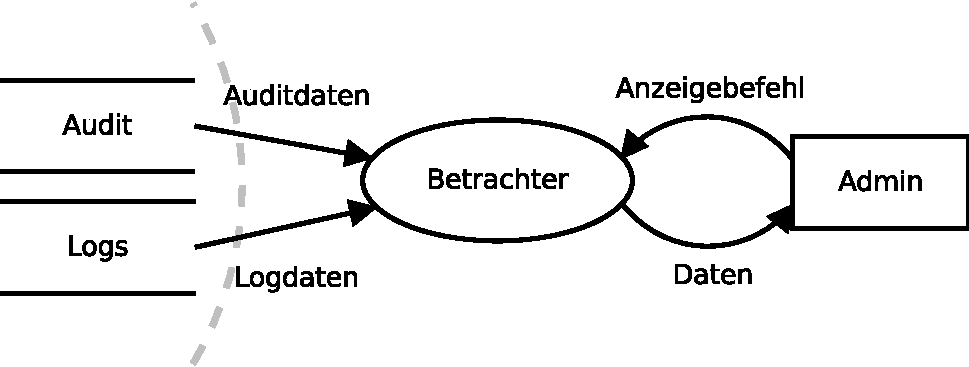
\includegraphics[scale=0.7]{images/dfd_logs.pdf}
\caption{DFD Logdaten Auswertung}
\label{fig:dfd_logs}
\end{figure}

\paragraph{Gefährdungen identifizieren}
Abbildung~\ref{fig:dfd_logs_threat} zeigt die Gefährdungen der einzelnen Beteiligten. Sabotage ist ein Aspekt der bei Log- und Audit-Dateien gegeben ist, den diese enthalten Informationen, die auf einen Angriff schließen lassen. Versucht ein Angreifer, beispielsweise per Bruteforce-Angriff das Passwort eines Benutzers herauszufinden, dann sind im Audit die fehlgeschlagenen Authentifizierungsversuche aufgezeichnet. Sollte dieser geglückt sein und der Benutzer hat Rechte das Audit zu verändern, kann der Angreifer seine Spuren verwischen. Ein anderer Angreifer könnte versuchen Schwachstellen in der Implementierung zu finden. Im Log würden dadurch zahlreiche Fehlermeldungen entstehen. Durch entfernen dieser kann er sicherstellen, dass eine eventuelle Sicherheitslücke unentdeckt bleibt. Der zweite Aspekt für Log- und Audit-Daten ist die Informationspreisgabe, da in beiden sensitive Daten enthalten sein können, welche Unberechtigte nicht einsehen dürfen. Informationspreisgabe ist auch für den Betrachter zu berücksichtigen, dieser darf Daten nur für Administratoren anzeigen. Zudem unterliegt er der Personifikation, indem der eigentliche Betrachter mit Schadcode modifiziert wurde und nun vorgibt, der Ursprüngliche zu sein. Auch der Administrator unterliegt der Personifikation, indem ein Angreifer in Besitz der Berechtigungsnachweise kommt. Zusätzlich muss die Datenwäsche berücksichtigt werden. Zwar kommen Log- und Audit-Daten von vertrauenswürdigen Quellen, die Daten enthalten allerdings Inhalte aus nicht vertrauenswürdigen Quellen. Daher sollten diese mit Vorsicht betrachtet werden. Ist der Betrachter, beispielsweise eine Web-Anwendung, dann ist es wichtig in den Daten nach JavaScript-Inhalten zu suchen und diese von einem Sanitizer entfernen zu lassen \footnote{Angriff erfolgreich durchgeführt an https://github.com/nlaplante/syslogng-web}.

\begin{figure}[htbp]
\centering
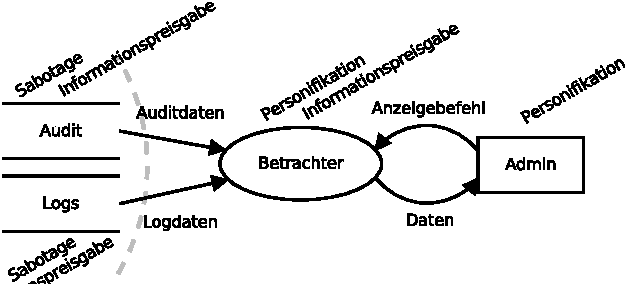
\includegraphics[scale=1.2]{images/dfd_logs_threats.pdf}
\caption{DFD Logdaten Gefährdungen}
\label{fig:dfd_logs_threat}
\end{figure}

\paragraph{Maßnahmen}

Aus den Gefährdungen ergeben sich folgende Maßnahmen, welche zur Sicherung der Informationsflüsse durchgeführt werden müssen. Log- und Audit-Daten dürfen in einer Datei oder Datenbank abgelegt werden, die ausschließlich vom Systembenutzer für Logging und Auditing beschrieben und modifiziert wird. Dabei wird angenommen, dass Datei-/Datenbankzugriffsmechanismus, sowie Systemauthentifizierung nicht komprimiert sind. Das Betrachten der Daten darf nur durch einen Administrator geschehen, dabei wird angenommen, dass der Betrachter nicht von einem Angreifer modifiziert wurde. Ist der Betrachter eine Web-Anwendung, benötigt er eine Authentifizierung, die mit der Systemauthentifizierung integriert ist. Log- und Audit-Daten müssen vor der Darstellung, durch einen Sanitizer, von schadhaften Inhalten befreit werden. Wurden, solche Daten entfernt, muss der Administrator darauf hingewiesen werden. Der Administrator, weist sich durch seinen Berechtigungsnachweis aus, dieser wird, von Ihm, vor fremden Zugriff geschützt. Weiterhin erfolgt erneut die Annahme, dass die Systemauthentifizierung nicht komprimiert wurde. Für alle Maßnahmen wird zudem angenommen, dass die Implementierung vollständig und korrekt ist.

\section{HTTP-Anfrage} \label{sec:model_http}

Eingehende Verbindungen sollen ausschließlich über HTTP/S erfolgen. Zu diesem Zweck wurde das RestGateway entwickelt, über welches auf den Marktrechner zugegriffen werden kann. 

\paragraph{Informationsfluss}

In Abbildung~\ref{fig:dfd_http} wird der Informationsfluss über das RestGateway gezeigt. Dabei fließen die Daten durch drei Vertrauensgrenzen. Sowohl RestGateway, als auch LanGateway fungieren als Datenproxy. Beide leiten die Anfragedaten ohne Validierung der Inhalte weiter. Deswegen muss darauf geachtet werden, dass ein Angreifer kein Datenwäsche durchführen kann. Das RestGateway arbeitet weiterhin als Wrapper, unterschiedliche Abfragen werden anhand der URL unterschieden und in entsprechende TCP-CAN-Telegramme übersetzt. Die URL-Parameter einer Anfrage, werden vom RestGateway auf einen gültigen Wertebereich überprüft. Die Antwort auf eine solche Anfrage sind menschenlesebare interpretierte Inhalte.

\begin{figure}[htbp]
\centering
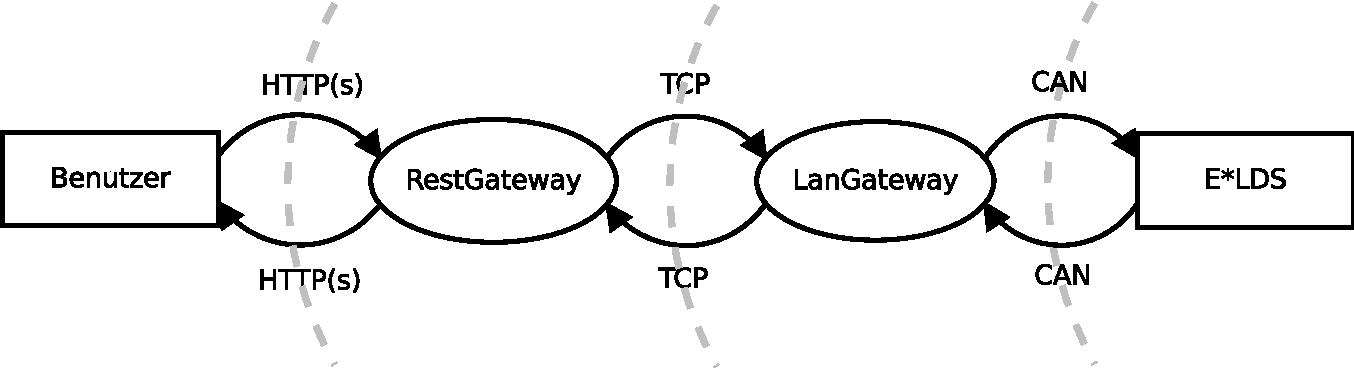
\includegraphics[scale=0.6]{images/dfd_http.pdf}
\caption{DFD HTTP-Anfrage}
\label{fig:dfd_http}
\end{figure}

\paragraph{Gefährdungen identifizieren}

In Abbildung~\ref{fig:dfd_http_threat} sind die Bedrohungen, in den vier Kategorien, aufgezeigt. Der Benutzer unterliegt der Gefahr der Personifizierung, durch stehlen der Berechtigungsnachweise. Dazu werden Phishing-Attacken genutzt, wobei versucht wird Benutzern, durch Personifikation eines legitimen Service, die Berechtigungsnachweise zu entwenden. Diese Angriffe geschehen meist per E-Mail oder Telefon. Da kein Nutzer die Log- und Audit-Daten verändern darf, besteht hierdurch keine Gefährdung durch Disput, da der Zugriff im Audit dokumentiert ist und später nachvollzogen werden kann. Ebenso unterliegen RestGateway und LanGateway der Personifikation, indem an ein Angreifer die Anfrage, über DNS-Spoofing, abfängt und weiterleitet. Dadurch wird er zum Man-in-the-Middle und kann die Unterhaltung mitverfolgen. Gleichzeitig ist dadurch die Informationspreisgabe gegeben. Der Angreifer kann, als Man-in-the-Middle, zum Saboteur werden. In dieser Funktion hat er die Möglichkeit Daten zum Marktrechner oder zum Kunden zu sabotieren. Die vierte Bedrohung, welche durch die Netzwerkkommunikation gegen ist, ist der Denial of Service. Diese Gefährdung kann den Marktrechner komplett außer Gefecht setzten, indem der RestGateway oder LanGateway Prozess dauerhaft mit Anfragen überlastet wird.

\begin{figure}[htbp]
\centering
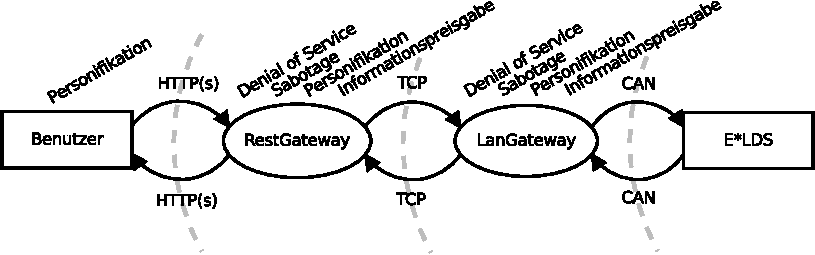
\includegraphics[scale=1]{images/dfd_http_threat.pdf}
\caption{DFD HTTP-Gefährdungen}
\label{fig:dfd_http_threat}
\end{figure}

\paragraph{Maßnahmen}

An Berechtigungsnachweise von Benutzern zu gelangen, ist für einen motivierten Angreifer, durch Phishing-Attacken möglich. Unter dieser Annahme, wird festgelegt, dass ungewöhnliche Login-Muster, in den Audit-Daten erkannt werden müssen. Zum Beispiel, wenn sich ein Benutzer, innerhalb weniger Minuten, von unterschiedlichen physikalischen Orten verbindet. Ebenso ist es keine Seltenheit, dass Benutzer ihren Berechtigungsnachweis vergessen, daher muss es eine Möglichkeit geben diesen sicher, schnell zurückzusetzen. Die Zurücksetzung per Telefon ist, beispielsweise nicht sicher, da man den Gesprächspartner nicht authentifizieren kann. Um RestGateway und LanGateway durch einen Man-in-the-Middle zu schützen, empfiehlt der BSI, statt DNS-Namen, IP-Adressen zu verwenden \cite{bsi_m559} und eine Ende-zu-Ende Verschlüsselung der Kommunikationsinhalte soll für weitere Authentizität sorgen. Die Verschlüsselung beziehungsweise Entschlüsselung, darf nicht dazu führen, dass der Marktrechner für längere Zeit ausgelastet wird. Da eine Denial of Service Attacke genau dies beabsichtigt, darf der Marktrechner, aus dem Internet, nur über einen Reverse Proxy erreichbar sein. Die Authentifizierung, welche in Abschnitt~\ref{sec:analysis_measures} gefordert wird, muss über drei Vertrauensgrenzen sichergestellt werden. Um die Gefährdungen, die durch die Schnittstellen und genutzten Protokolle entstehen zu reduzieren, sollten die Funktionen des LanGateway in das RestGatway integriert werden. Ein externes RestGateway würde, anstatt des LanGateway, mit dem internen RestGateway kommunizieren, welches dann lediglich als Proxy fungiert. Alternativ muss sichergestellt werden, dass das LanGateway ausschließlich lokal, über die Loopback-Addresse (127.0.0.1), erreichbar ist. Die Daten fließen durch mehrere Vertrauensgrenzen, dabei sollte jedoch an keine Stelle angenommen, dass diese vom jeweiligen Vorgänger durch Schadcode befreit worden sind. Das jeweilige Software-Module, hat dafür sorge zu tragen, dass Schadcode der Ihn schädigen kann, von einem Sanitizer bereinigen zu lassen. Dadurch wird der Schadcode zwar bis zum entsprechenden Modul mitgenommen, diese geht jedoch davon aus, dass die Inhalte nicht vertrauenswürdig sind.

\begin{comment}
\begin{figure}[htbp]
\centering
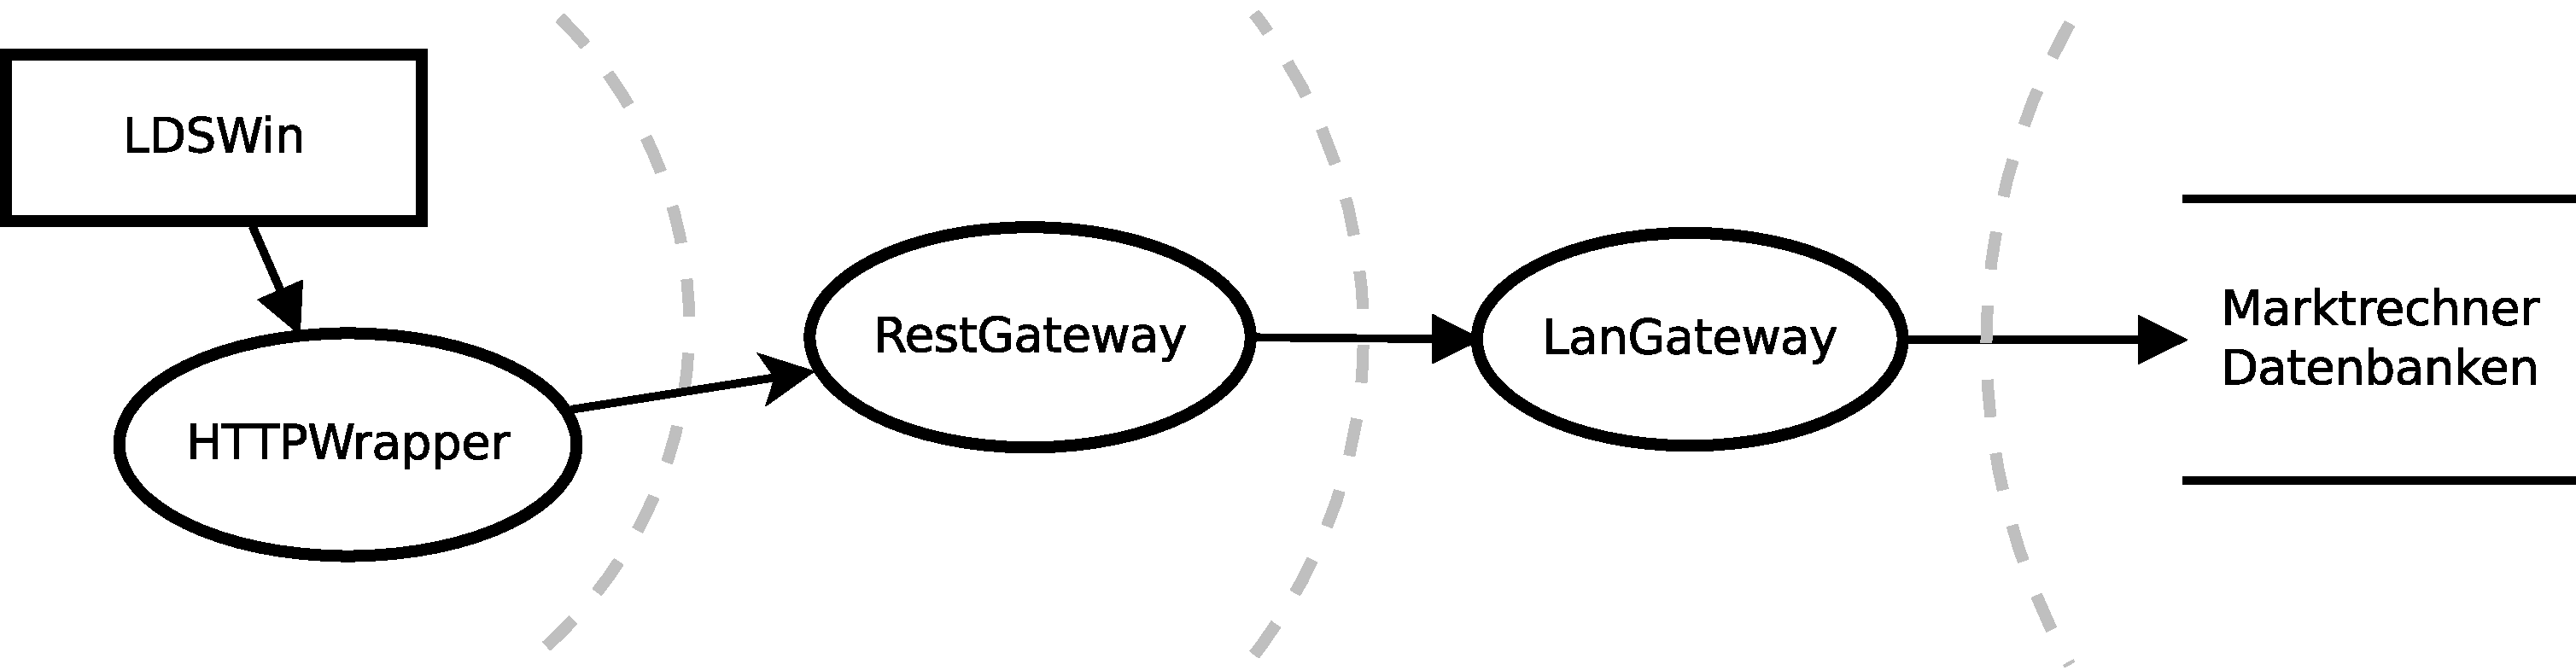
\includegraphics[scale=0.24]{images/dfd_http_legacy.pdf}
\caption{DFD HTTP-Anfrage Legacy-System}
\label{fig:dfd_http_leg}
\end{figure}
\end{comment}

\chapter{Sicherheitsdesign} \label{chap:design}
\epigraphhead[70]{\epigraph{The user's going to pick dancing pigs over security every time.}{\textit{Bruce Schneier}}}

In diesem Kapitel werden die Erkenntnisse und Maßnahmen aus den Kapiteln Bedrohungsanalyse (\ref{chap:threat_analysis}) und Bedrohungsmodellierung (\ref{chap:threat_modelling}) genommen, um ein technologisch unabhängiges Design eines Sicherheitskonzeptes zu erstellen. Die Schwerpunkte werden dabei auf dem Authentifizierungsmechanismus und der Distribution und Verwaltung von Berechtigungsnachweisen liegen.

\section{Kryptographie} \label{sec:design_crypto}

Kryptographie ist für die Authentifizierung und die Verschlüsselung der Daten unerlässlich. Dabei spielt der eingesetzte Algorithmus keine Rolle, solange dieser ordentlich entwickelt und unabhängig geprüft wurde, denn kein Angreifer wird die Kryptographie als Angriffsziel wählen [\ref{sec:security_conzept}]. Stattdessen werden diese versuchen, alle anderen Komponenten des Systems zu attackieren. Bei der Auswahl eines Algorithmus sollte darauf geachtet werden, dass dieser effizient auf dem Marktrechner zu benutzen ist. Des Weiteren sollen die Algorithmen Perfect Forward Security (PFS) bieten, damit aufgenommene Inhalte nicht zu einem später Zeitpunkt, beispielsweise durch erlangen des Schlüssels, kompromittiere werden können. 

\section{Komponentenarchitektur}

In der Komponentenarchitektur sind die Maßnahmen aus Bedrohungsanalyse und Bedrohungsmodellierung berücksichtigt. (Abbildung~\ref{fig:comp_arch}). Komponenten für die Authentifizierung sind nicht enthalten, diese werden im folgenden Abschnitt~\ref{sec:design_auth}, basierend auf dem Verfahren, hinzugefügt. Das RestGateway des Marktrechners funktioniert als Server für Anfragen. Da der Marktrechner als Server nur geringe Ressourcen zur Verfügung hat wird die Maßnahme, aus Abschnitt~\ref{sec:model_http}, einen Reverse Proxy einzusetzen, umgesetzt. Dieser schützt den Marktrechner vor Überlastung, durch zu viele Anfragen aus dem Internet. Zusätzlich wird das RestGateway mit dem LanGateway integriert, um eine unnötige Schnittstelle zu eliminieren. Der Mediator wird durch eine externes RestGateway realisiert. An dieses stellt der Benutzer seine Abfrage, welche für diesen transparent die Anfrage an den eigentlichen Marktrechner weiterleitet. Durch diese Doppelrolle wird nur eine Implementierung für die Authentifizierung zwischen den RestGateways benötigt. Auch die Flexibilität des RestGateways, schnell und einfach neue Funktionen testen zu können, bleibt dadurch erhalten. 

\begin{figure}[htbp]
\centering
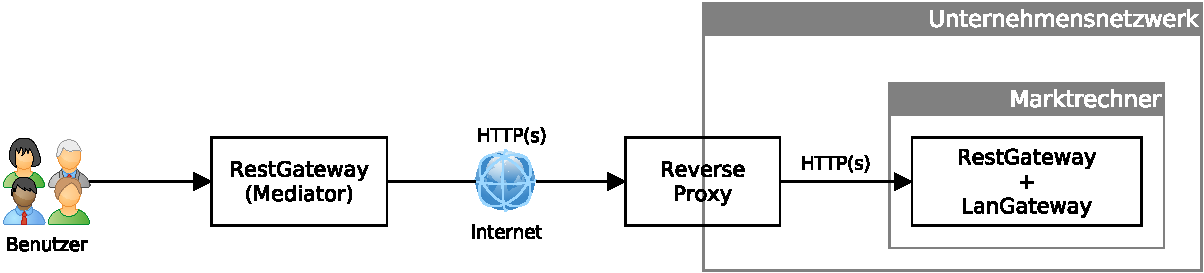
\includegraphics[scale=0.5]{images/design_architekture.pdf}
\caption{Komponentenarchitektur}
\label{fig:comp_arch}
\end{figure}

\section{Authentifizierung} \label{sec:design_auth}

Die Authentifizierung wird an zwei Stellen benötigt. Zum einen damit sich der Benutzer dem Mediator gegenüber ausweisen kann und zum anderen, damit Mediator und Marktrecher gegenseitig ein Vertrauensverhältnis aufbauen können.

\subsection{Benutzerauthentifizierung} 

Die einseitige Authentifizierung gegenüber dem Benutzer hat administrative Gründe. Den obwohl der Einsatz einer gegenseitigen Authentifizierung aus sicherheitstechnischen Gründen durchaus ratsam ist, so ist die Administration von Personen, die einer hohen Fluktuation unterliegen, schwierig und dadurch sehr kostenintensiv. Abbildung~\ref{fig:design_authu} zeigt eine Integration des RestGateway mit verschiedenen Authentifizierungslösungen. Unternehmen haben in der Regel eine existierende Lösung, um Benutzer zu authentifizieren. Das, als Mediator fungierende, RestGateway soll deshalb mit diesen Lösungen integrieren werden. Dadurch muss keine eigene Lösung zur Benutzerauthentifizierung implementiert werden, wodurch sich das RestGateway auf seine Kernaufgabe konzentrieren kann. Zudem sind die Systeme, wie etwa LDAP oder Radius, seit Jahren im Einsatz und dadurch verlässlicher als eine eigene Lösung. Ein weiterer Vorteil ist die Vermeidung von Redundanzen, da die Benutzer im Fernservicenetzwerk zentral verwaltet werden. Hinzu kommt das Poltische Umfeld, indem viele Unternehmen eigene Richtlinien an Authentifizierungsmaßnahmen haben, beispielsweise Passwortregeln oder zwei Faktor-Anmeldung mit Hardwaretoken, welche einen enormen Implementierungsaufwand für das RestGateway bedeuten würde.

\begin{figure}[htbp]
\centering
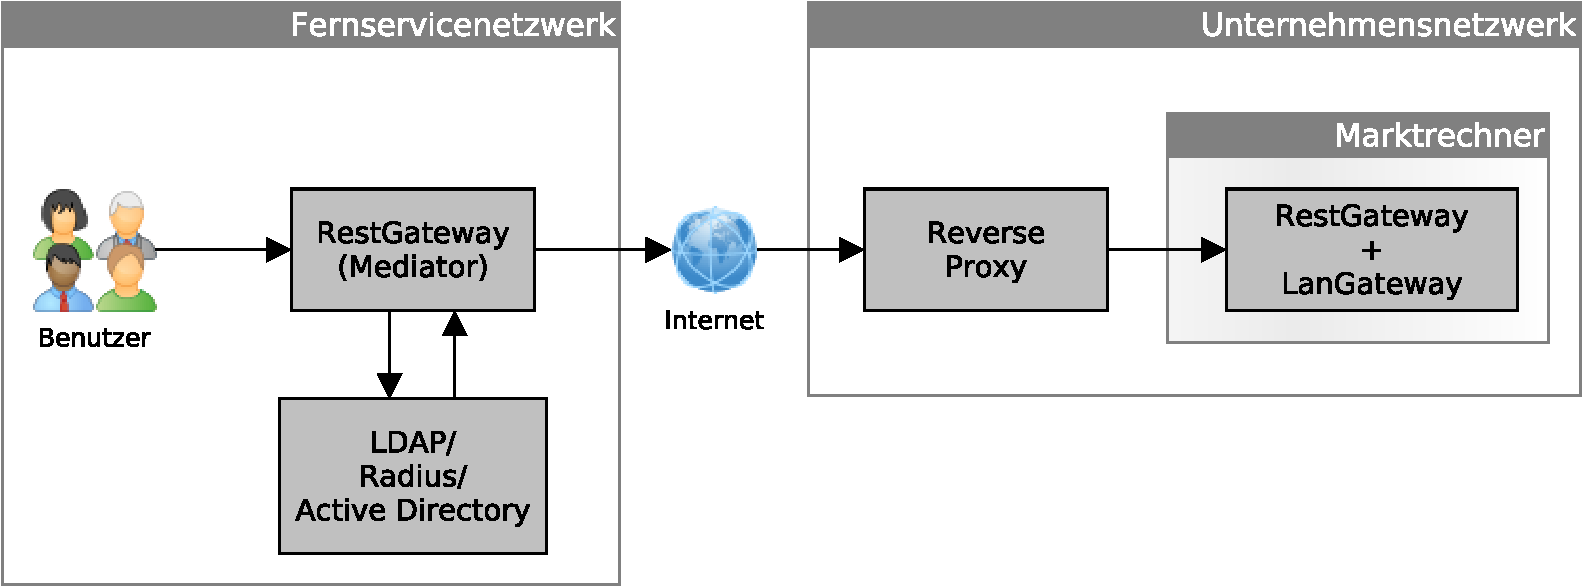
\includegraphics[scale=0.5]{images/design_architecture_auth_user.pdf}
\caption{Komponentenarchitektur}
\label{fig:design_authu}
\end{figure}

\subsection{Maschine-to-Maschine Authentifizierung}

Die gegenseitige Authentifizierung von Mediator und Marktrechner, sollte nicht durch Passwörter geschehen, da diese zwangsläufig im Klartext, in einer Konfigurationsdatei gespeichert werden müssen. Bei der Maschine-to-Maschine (M2M) Kommunikation ist es daher sinnvoll schlüsselbasierende oder zertifikatbasierende Kryptosysteme zu nutzen. Im folgenden Abschnitt wird das Design einer asymmetrischen Authentifizierung für die M2M-Kommunikation genommen. Symmetrische Authentifizierung spielt hier keine Rolle, da diese zwingend einen zweiten Kanal für den Schlüsselaustausch benötigt.

\subsubsection{Key Continuous Management}

Die Kryptographie von Authentifizierungslösungen wurde vor Jahrzehnten entworfen und ist dementsprechend erprobt. In Abschnitt~\ref{sec:design_crypto} wurde bereits erläutert, dass diese keine Schwachstelle in der Authentifizierungskette darstellt. Damit die Kryptographie funktioniert, werden Schlüssel benötigt. Die primäre Problemstellung bei der Schlüsselverwaltung ist---Wie gelangt ein Schlüssel vom Erzeuger zu den vorgesehenen Empfängern? Das populärste Modell der Schlüsselverteilung ist das "Schlüssel fallen aus dem Himmel"-Modell. Es ist deshalb so weit verbreitet, weil durch die Komplexität des Problems, Entwickler von Sicherheitsprotokollen es gerne ignorieren und jemand anderem zuschieben. Ein Konzept, das nicht dem "Schlüssel fallen aus dem Himmel"-Modell unterliegt, ist das der Schlüsselkontinuität. Ihm zugrunde liegt das Konzept der Beständigkeit, dass bedeutet anhand des Schlüssel kann überprüft werden, ob die Entität, mit welcher gestern kommuniziert wurde auch heute noch dieselbe ist. Die Schlüsselkontinuität unterliegt allerdings einer Schwachstelle, den beim initialen Austausch ist eine MITM-Attacke möglich. Ein Angreifer hat dementsprechend exakt eine Chance die Verbindung zu kompromittieren. Wenn er zu diesem Zeitpunkt die Attacke nicht durchführen kann, hat er seine Chance vertan. Ein derartiger Angriff ist nicht auszuschließen, jedoch ist das Wahrscheinlichkeit sehr gering und daher das Risiko akzeptable.

\subsubsection{Authentifizierungsprozess}

Bei der asymmetrische Authentifizierung, ist es möglich den Öffentlichen Schlüssel oder ein selbst-signiertes Zertifikat, über einen unsicheren Kommunikationskanal auszutauschen. In Abbildung~\ref{fig:design_authm2m} ist das Vorgehen einer Authentifizierung, die der Schlüsselkontinuität genügt, gezeigt. Der initiale Austausch unterliegt dem erwähnten Risiko einer MITM-Attacke, deshalb empfiehlt die Schlüsselkontinuität einen Fingerprint zu erstellen und diesen über einen zweiten Kanal auszutauschen. Anhand des Fingerprints kann festgestellt  werden, ob der Schlüssel während des Austausches manipuliert wurde. Nachdem der Schlüssel durch den Fingerprint verifiziert wurde, muss dieser mit einem Identifikator (ID), welcher die Entität des Schlüsselerzeugers eindeutig nachweist, abspeichern werden. Die ID besteht, beispielsweise aus Domain und Port. Als weitere Sicherheitsmaßnahme dürfen IDs für den Fall, dass ein Angreifer lesenden Zugriff erhält, nur als Hash mit dem Schlüssel oder Zertifikat gespeichert. Der Fingerprint dient lediglich der Verifizierung und wird nicht mit abgespeichert.
Bei einer erneuten Verbindung überprüfen beide Teilnehmer, ob die Entität des Anderen mit dem bekannten Schlüssel übereinstimmt. Eine Authentifizierung ist, in diesem Fall, erfolgreich. 

\begin{figure}[htbp]
\centering
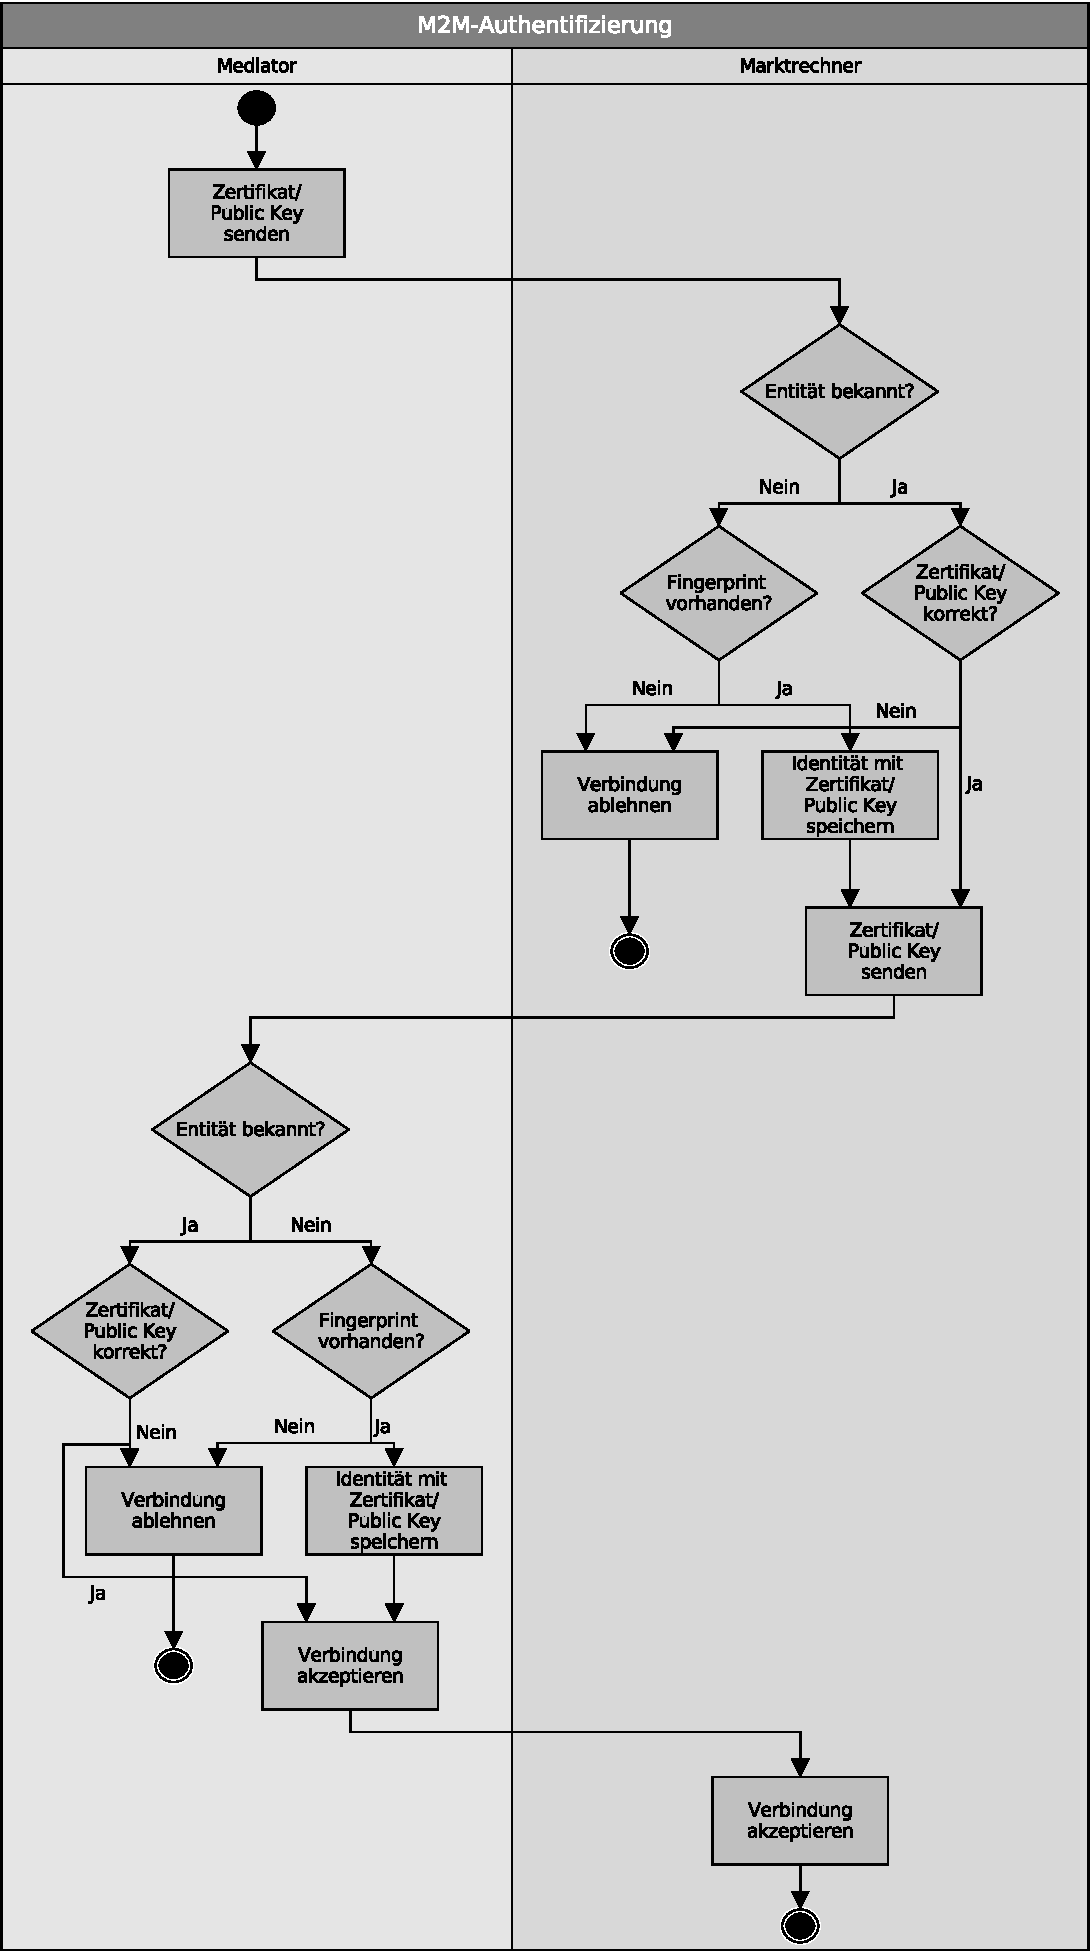
\includegraphics[scale=0.7]{images/design_architecture_auth_m2m_h.pdf}
\caption{M2M-Authentifizierung}
\label{fig:design_authm2m}
\end{figure} 

Protokolle die Ansätze des Key Continuous Management implementieren sind Secure Shell (SSH) und Pretty Good Privacy (PGP). SSH führt eine auf dem Öffentlichen Schlüssel basierenden Vergleich, der jedem Verbindungsaufbau durchgeführt wird. Bei jeder neuen SSH Verbindung wird auch ein Fingerprint generiert, welcher getauscht werden kann. Allerdings besitzt SSH kein Konzept Schlüssel auf geeignete Weise zu sichern und wieder einzuspielen, beispielsweise beim neu aufsetzen eines Servers. Zudem verbieten die meisten Firewalls SSH-Zugriffe aus dem Internet, weshalb es nicht als Protokoll in Frage kommt. PGP hingegen erfüllt alle Anforderungen an Key Continuous Management, wird jedoch fast ausschließlich für E-Mail Kommunikation genutzt. Für den Marktrechner soll HTTP beziehungsweise HTTPS genutzt werden, dieses verfügt jedoch nicht über ein Konzept zur Schlüsselkontinuität. Vielmehr vertraut es auf den Einsatz von Zertifizierungsstellen, welche ein Single-Point-of-Failure in der Authentifizierungskette sind. Des Weiteren ist für die Authentifizierung wichtig, dass leidlich der Zertifikatsinhaber und die Zertifizierungsstelle miteinander bekannt sind. Der Client, welcher die Zertifizierungsstelle zu Überprüfung des Zertifikates konsultiert, hat zu dieser keine Beziehung. Damit HTTP(S) Schlüsselkontinuität unterstützt, gibt es zwei Möglichkeiten, zum einen anpassen des HTTP-Protokolls. Da HTTP weltweit auf allen Webservern eingesetzt wird, wäre dies eine extrem langwieriger Prozess mit sehr geringer Umsetzungswahrscheinlichkeit. Zum anderen bietet sich die Möglichkeit ein weiteres Protokoll auf HTTP zu implementieren. Dies ist nicht optimal, jedoch durchaus umsetzbar.

\subsection{Lokale Authentifizierung}

Die Authentifizierung lokal am CI4000 ist ausschließlich dem Eigentümer vorbehalten. Dieser soll in der Lage einen lokalen Zugriff für einem Partner, der die Anlage in Betrieb nimmt, überwacht und wartet, freizugeben. Für den Fernzugriff auf die Anlage können Verbindungen zu Mediatoren angelegt werden. Weitere Sonderauthentifizierungen sind in Abschnitt~\ref{sec:extra_auth} erläutert. Lokal über Mediator

\subsection{Sonderauthentifizierung} \label{sec:extra_auth}

Bei den Sonderauthentifizierungen handelt es sich, um explizit durch den Eigentümer oder dessen Vertreter, in Form eines Service-Partners (FSZ), ausgestellte Erlaubnis auf das System zuzugreifen.

\paragraph{Die zeitbeschränkte Authentifizierung} erlaubt es einem Benutzer für einen bestimmten Zeitraum, beispielsweise 24 Stunden, auf die Anlage zuzugreifen. 

\paragraph{Die Einmal-Authentifizierung} erlaubt es über einen generierten Schlüssel oder Passwort einmalig Zugriff auf den Marktrechner zu erlangen.

Die Umsetzung dieser Authentifizierungen kann auf zwei Ebenen erfolgen. Zum einen auf Benutzerlevel, dann werden über die am Mediator verknüpfte Benutzerverwaltung entsprechende Freigaben erteilt. Zum anderen im Marktrechner, im diesem Fall generiert der Marktrechner auf Anforderung eines Lokalen Administrators, beispielsweise des Eigentümer, einen Schlüssel über welchen sich einmalig oder zeitbeschränkt angemeldet werden kann. Der Mediator benötigt dazu die Möglichkeit, die Benutzerverwaltung zu übergehen und sendet den generierten Schlüssel an den Marktrechner. Ob der Zugriff dabei einmalig oder zeitbeschränkt ist, spielt für den Mediator keine Rolle. Beim Anlegen der Sonderberechtigung muss eine entsprechende Rolle für die Autorisierung angegeben werden. Der Mediator soll selbst keine Berechtigungsnachweise für Benutzer hinterlegt haben.

\section{Autorisierung}

Die Autorisierung der Benutzer erfolgt am Mediator und ist rollenbasiert. Bei der Authentifizierung verlässt sich der Mediator auf die verknüpfte Benutzerverwaltung. Diese teilt ihm die Rollen eines authentifizierten Benutzers mit. Die Rollen für die Autorisierung wurden in Abschnitt~\ref{sec:roles} benannt und sollen so umgesetzt werden. Vom Mediator  werden die Rollen an den Marktrechner gesendet, welcher daraufhin entsprechende Funktionen freigibt. Für die verschiedenen Rollen gelten bestimmte Einschränkungen, die im Folgenden erläutert werden.

\subsection{Rollen}

Der Inbetriebnehmer und der Projektierter sorgen dafür, dass eine Kälteanlage ihren Betrieb aufnehmen kann. Während der Inbetriebnahme dürfen ausschließlich diese beiden Rollen auf den Marktrechner zugreifen. Dazu müssen Sie lesend und schreiben auf das System zugreifen können. Nachdem ihre Tätigkeit abgeschlossen ist, geben Sie den Zugriff für andere Rollen frei. System-Analyst und Marktpersonal sollen nur lesenden Zugriff auf benötigte Funktionen erhalten. Die für Überwachung und Wartung zuständigen Rollen Service-Monteur und Fernservice-Mitarbeiter benötigen hingegen auch schreibenden Zugriff, um regulierend in die Anlage eingreifen zu können. Die Rolle des Herstellers ist eine Ausnahme, sie soll zu jeder Zeit vollen Zugriff erhalten können, jedoch ausschließlich, wenn dieser vorher durch die Fernservice-Zentrale oder den Eigentümer freigegeben wurde. Außerdem soll der Zugriff des Herstellers immer zeitlich begrenzt sein, beispielsweise für 24 Stunden.

Durch die Authentifizierung wird ein Vertrauensverhältnis mit booleschen Zuständen, nämlich Vertrauen und kein Vertrauen, erreicht. In der realen Welt ist Vertrauen allerdings selten boolesch, sondern baut sich langsam auf, beziehungsweise ab. Um ein derartiges gestaffeltes Vertrauensverhältnis herzustellen kann, beispielsweise angenommen werden, je öfter man mit derselben Entität bereits verbunden war, desto vertrauenswürdiger ist diese. Die Autorisierung könnte über ein mehrstufiges Vertrauen, beispielsweise das Recht Änderungen an der Anlage zu tätigen von einen Vertrauenswert abhängig machen, der erst nach drei Tagen erreicht werden kann. Ein Angreifer, der es schafft sich als Mediator auszugeben, müsste dann mehrere Tage aktiv das Netzwerk kompromittieren, bevor er das System manipulieren kann. Dadurch ist das Risiko entdeckt zu werden und die Wahrscheinlichkeit, dass die Beschützer den Angreifer enttarnen deutlich erhöht.

\section{Audit}



\chapter{Evaluation} \label{chap:evaluation}
\epigraphhead[70]{\epigraph{Wisdom consists in being able to distinguish among dangers and make a choice of the least harmful.}{\textit{Niccolo Machiavelli, The Prince}}}

Vorstellung und Evaluation der beonden Systeme WIBU und Radius anhand des Entwurfs oder Designs in Kapitel~\ref{chap:design}.

Sicherheitsdesign dient als Grundlage, an welcher die Produkte gemessen werden.

Kriterien:
* Installation - Voraussetzungen, Software, Hardware, Dokumentation
* Wartung - Hinzufügen, ändern oder löschen von Benutzern, Marktrechnern, (Mediatoren)
* Sicherheit - Eingesetzte Authentifizierung, Algorithmus geprüft? --- Verschlüsselung der Daten, Algorithmus geprüft?
* Effizienz - Mechanismus 
                                            
\section{WIBU Systems}

\section{Radius}

\section{Gegenüberstellung}

\chapter{Implementierung} \label{chap:implementation}

Beschreibung der Implementierung, der aus der Evaluation gewählten Lösung. Was wenn keine der beiden Lösungen passt?

* Performance von bestimmten Algorithmen testen---libsodium als Testlibrary 
* Prototyp---Implementierung von WIBU oder Radius, alternative KCM mit libsodium

\chapter{Fazit}

%%%%%%%%%
% TABLE %
%%%%%%%%%
\begin{comment}
\begin{table}[htbp] % htbp ~ here, top, bottom, page
\centering
\begin{tabular}{|r|c|l|l|}
\hline
\textbf{Name} & \textbf{Adresse} & \textbf{Wohnort} & \textbf{Telefon} \\ 
\hline\hline
Susi Sinnlos & Eichenstrasse 5 & 12345 Unterstadt & 24927749242 \\
Horst Kurz & Schnellweg 17 & 42420 Rapid & 999 \\\hline
Jochanaan Leuchtentrager & Hochstraße zu & 666 Hell & 1-800-33845\\\hline
\end{tabular}
\caption{Adressliste}
\label{tab:meinetab}
\end{table}

%%%%%%%%%
% ITEMS %
%%%%%%%%%
\begin{itemize}
\item Jede Tabelle, jedes Bild und jedes Listing ist ein Fließobjekt.
\item Zentrieren Sie Bilder und Tabellen.
\item Jedes Fließobjekt hat eine Bildunterschrift (Caption) mit
  einem Label und wird im Text passend referenziert.
\end{itemize}
\end{commit}

%%%%%%%%%%
% IMAGES %
%%%%%%%%%%

\begin{wrapfigure}{r}{6cm}
  \centering
  \includegraphics[width=4cm]{gnu}
  \caption{GNU-Logo~\cite{gnulogo,fal}}
  \label{fig:gnu}
\end{wrapfigure}

\begin{figure}[htb]
\centering
\includegraphics[width=.6\textwidth]{zeichnung} % pdflatex ohne Endung
\caption{Die tolle Konzeptzeichnung}
\label{fig:tk}
\end{figure}

\begin{comment}
\begin{figure}[htb]
\centering
\subfloat[Vektor]{\label{fig:vektor}
  \includegraphics[width=.3\textwidth]{zeichnung}}
\subfloat[JPG]{\label{fig:jpg}
  \includegraphics[width=.3\textwidth]{zeichnungjpg}}
\subfloat[PNG]{\label{fig:png}
  \includegraphics[width=.3\textwidth]{zeichnungpng}}
\caption{Die tolle Konzeptzeichnung in unterschiedlichen Formaten}
\label{fig:tk2}
\end{figure}

\begin{figure}[htb]
\centering
\includegraphics[width=.4\textwidth]{zeichnungdraft} 
\caption{Die tolle Konzeptzeichnung als Draft}
\label{fig:tkdraft}
\end{figure}

%%%%%%%%%%%
% LISTING %
%%%%%%%%%%%


\begin{listing}[htbp]
\lstset{basicstyle=\rmfamily, columns=[l]flexible, mathescape=true, showstringspaces=true, numbers=none, language=java}
\begin{lstlisting}
public static int ggt(int x, int y) {
    while (x != 0) {
      int h = x;
      x = y%x;
      y = h;
    }
    return y;
}
\end{lstlisting}
\caption{ggT --- Java}
\label{code:ggtjava}
\end{listing}
\end{comment}

\newpage

% Listen wenn überhaupt ans Ende und nicht an den Anfang.
% Meist ist das aber unnötig.
%\listoffigures % Liste der Abbildungen 
%\listoftables % Liste der Tabellen
% \newpage

\bibliographystyle{plain} % Literaturverzeichnis
\begin{btSect}{thesis} % mit bibtopic Quellen trennen
\section*{Literaturverzeichnis}
\btPrintCited
\end{btSect}
\begin{btSect}{online}
\section*{Online-Quellen}
\btPrintCited
\end{btSect}
% dann mit "bibtex thesis1" und "bibtex thesis2" arbeiten

\end{document}
;;; Local Variables:
;;; ispell-local-dictionary: "de_DE-neu"
;;; End:
